\documentclass[a4paper,12pt]{article}
\usepackage[T1]{fontenc}
\usepackage[polish]{babel}
\usepackage{amsmath, amssymb}
\usepackage{mathtools}
\usepackage{physics}
\usepackage{graphicx}
\usepackage{float}
\usepackage{geometry}
\usepackage{parskip}
\usepackage{tikz}
\usepackage[hidelinks]{hyperref}
\geometry{left=25mm, right=25mm, top=25mm, bottom=25mm}
\graphicspath{{images/}{./}}

\begin{document}

\title{Podstawy mechaniki kwantowej}
\author{Notatki z wykładu}
\date{\today}
\maketitle
\tableofcontents

\section{Historia powstania fizyki kwantowej}

\subsection{Zapomnijmy o mechanice klasycznej}
Związek z nią będzie jasny, kiedy pójdziemy głębiej w teorię.

\subsection{Promieniowanie ciała doskonale czarnego}
Eksperyment Stefana-Boltzmanna (1878) badał promieniowanie cieplne emitowane przez ciało doskonale czarne.
Ciało doskonale czarne to obiekt, który pochłania całe promieniowanie i emituje je zgodnie z temperaturą.
\begin{figure}[H]
    \centering
    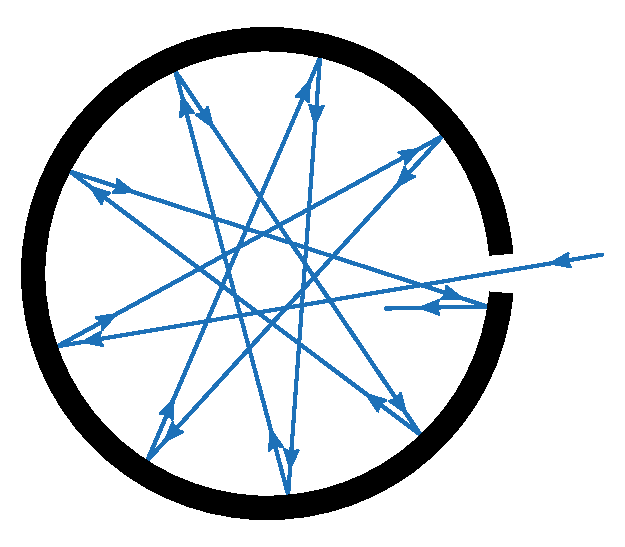
\includegraphics[width=0.3\textwidth]{blackbody}
    \caption{Ciało doskonale czarne. \textit{Źródło: Wikipedia}}
    \label{fig:blackbody}
\end{figure}

Pokazano, że całkowita energia wypromieniowywana przez takie ciało jest proporcjonalna do czwartej potęgi jego temperatury absolutnej
\begin{equation*}
    R(T) = \sigma T^4,
\end{equation*}
gdzie $R$ to moc promieniowania na jednostkę powierzchni, $T$ to temperatura w kelwinach, a $\sigma$ to stała Stefana-Boltzmanna.

Całkowita moc promieniowania to
\begin{equation*}
    R(T) = \int_0^\infty \rho(\lambda, T) d\lambda,
\end{equation*}
gdzie $\lambda$ to długość fali, a $\rho(\lambda, T)$ to spektralna funkcja rozkładu.

W 1893 Wien zauważył, że spektralna gęstość promieniowania nie zależy od $\lambda$ i $T$ osobno, ale od ich iloczynu $\lambda T$
\begin{equation*}
    \rho(\lambda, T) = \lambda^{-5} f(\lambda T).
\end{equation*}

\subsection{Prawo Rayleigha-Jeansa}
W klasycznej elektrodynamice, promieniowanie elektromagnetyczne opisane jako fale stojące daje rozkład energii w funkcji długości fali.
Liczba takich fal o długości od $\lambda$ do $\lambda + d\lambda$ to
\begin{equation*}
    \rho(\lambda, T) = \frac{8\pi}{\lambda^4} \cdot \bar{\epsilon},
\end{equation*}
gdzie $\bar{\epsilon}$ to średnia energia takiej fali.
Wzór ten jest dokładny dla długich fal, ale prowadzi do problemu z ,,katastrofą ultrafioletową'' przy krótkich falach, co zostało skorygowane przez teorię kwantową Plancka.

\begin{figure}[H]
    \centering
    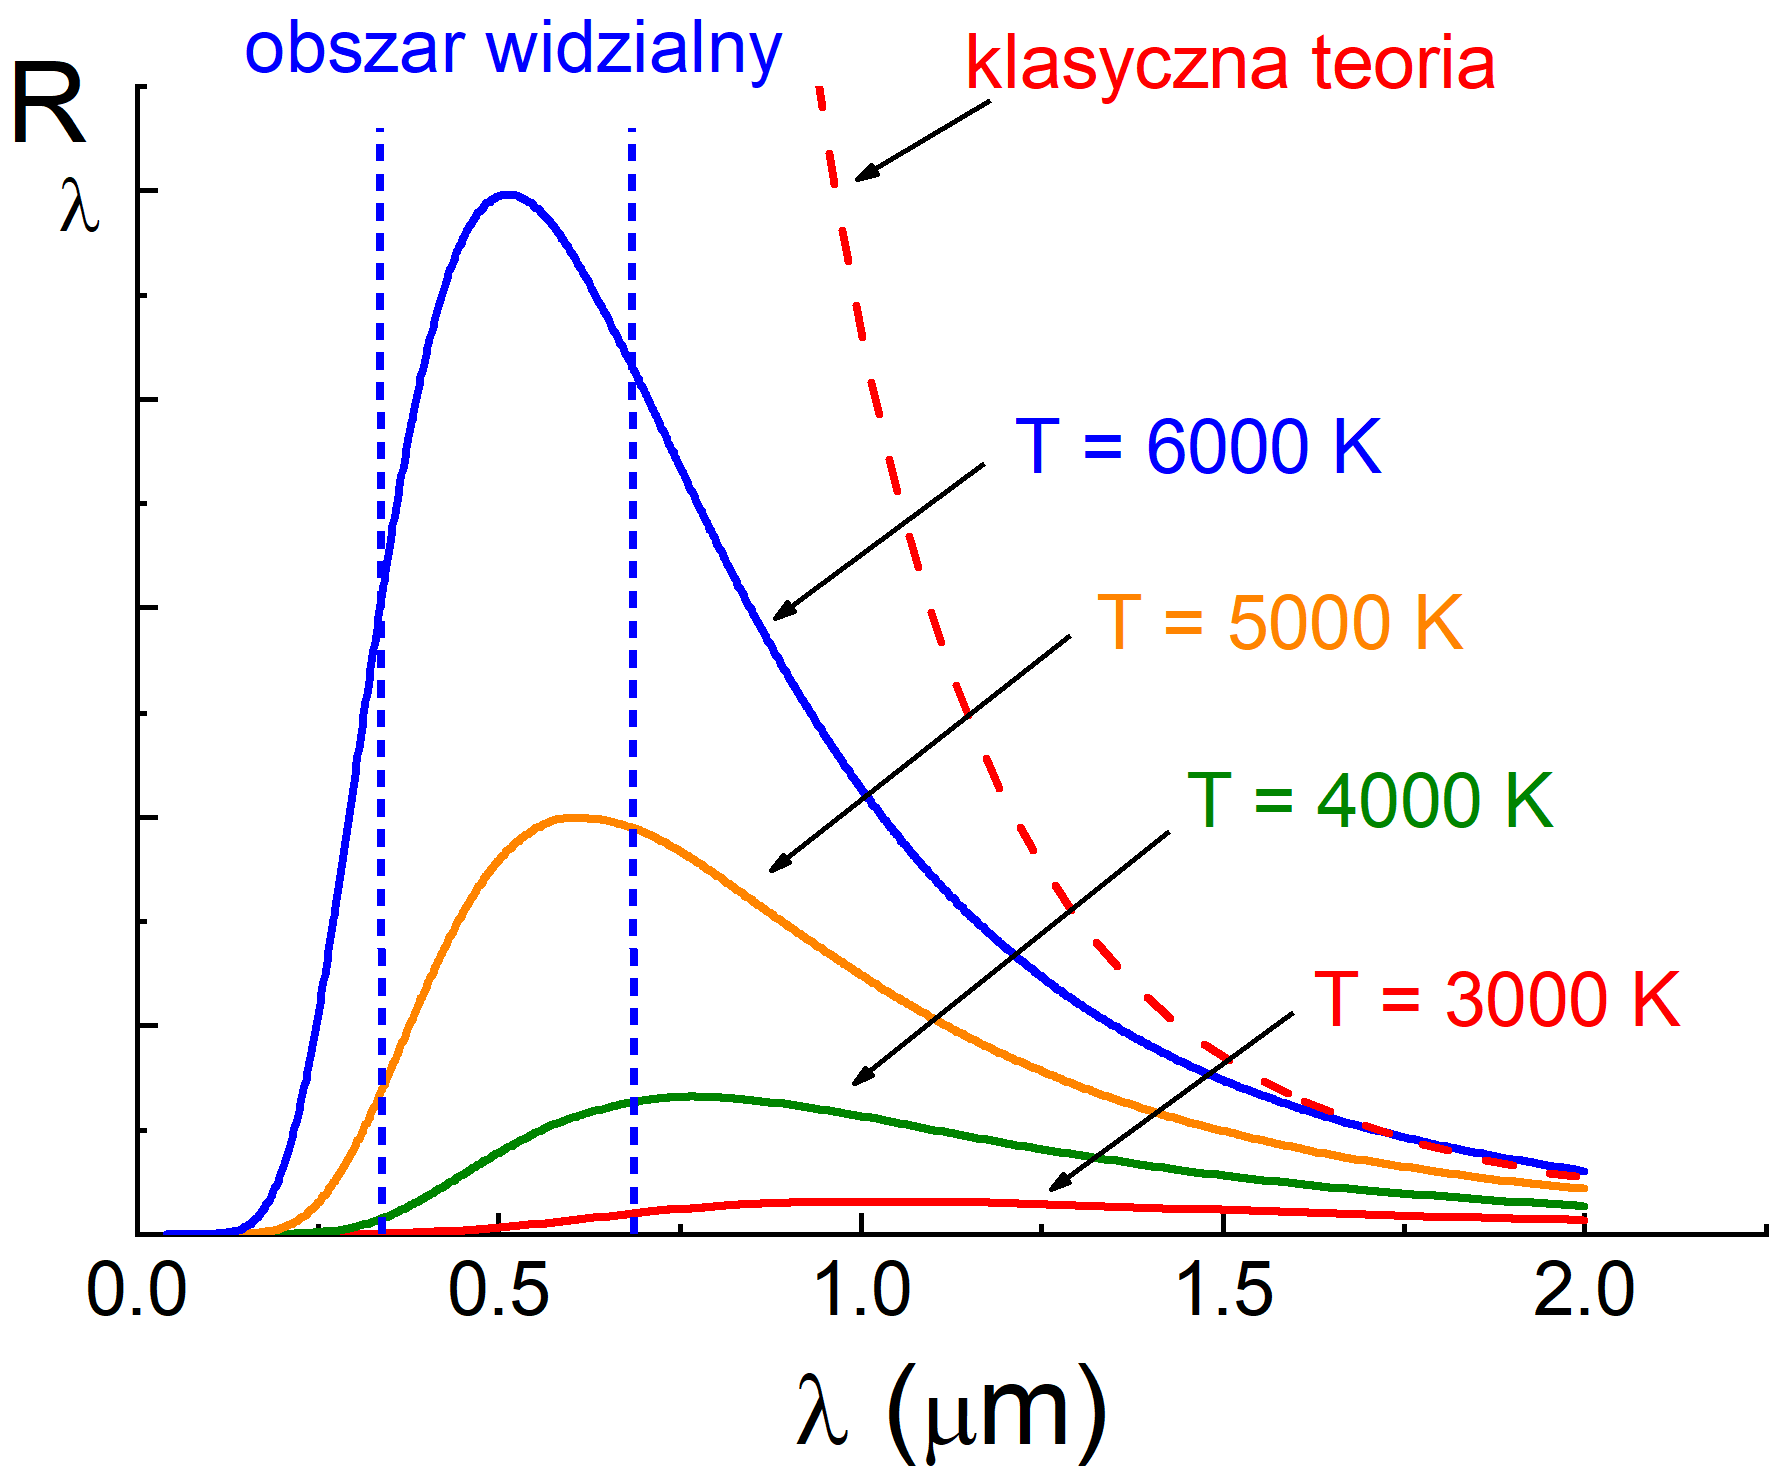
\includegraphics[width=0.5\textwidth]{widmo-promieniowania}
    \caption{Widmo promieniowania ciała doskonale czarnego w wybranych temperaturach. \textit{Źródło: e-Fizyka, AGH}}
    \label{fig:widmo-promieniowania}
\end{figure}

\subsection{Teoria kwantowa Plancka}
W 1900 roku Planck zaproponował, że ciała emitują światło w postaci kwantów ($\epsilon = n\epsilon_0$)
\begin{equation*}
    \bar{\epsilon} = \frac{\sum\limits_{n=0}^{\infty} n\epsilon_0 \exp(-\frac{n\epsilon_0}{kT})}{\sum\limits_{n=0}^{\infty} \exp(-\frac{n\epsilon_0}{kT})} = \cdots = \frac{\epsilon_0}{\exp(\frac{\epsilon_0}{kT}) - 1},
\end{equation*}
gdzie \(\epsilon_0 = h \nu = \frac{h c}{\lambda}\) jest energią jednego kwantu promieniowania.

Z tego wyrażenia Planck otrzymał rozkład promieniowania w funkcji długości fali, który ma postać
\begin{equation*}
    \beta(\lambda, T) = \frac{8\pi hc}{\lambda^5} \cdot \frac{1}{\exp(\frac{hc}{k\lambda T}) - 1},
\end{equation*}
Wzór ten zgadza się z wynikami eksperymentalnymi, eliminując problem ,,katastrofy ultrafioletowej''.

\subsection{Efekt fotoelektryczny}
Efekt fotoelektryczny to zjawisko emisji elektronów z powierzchni metalu pod wpływem padającego na niego światła.

\begin{figure}[H]
    \centering
    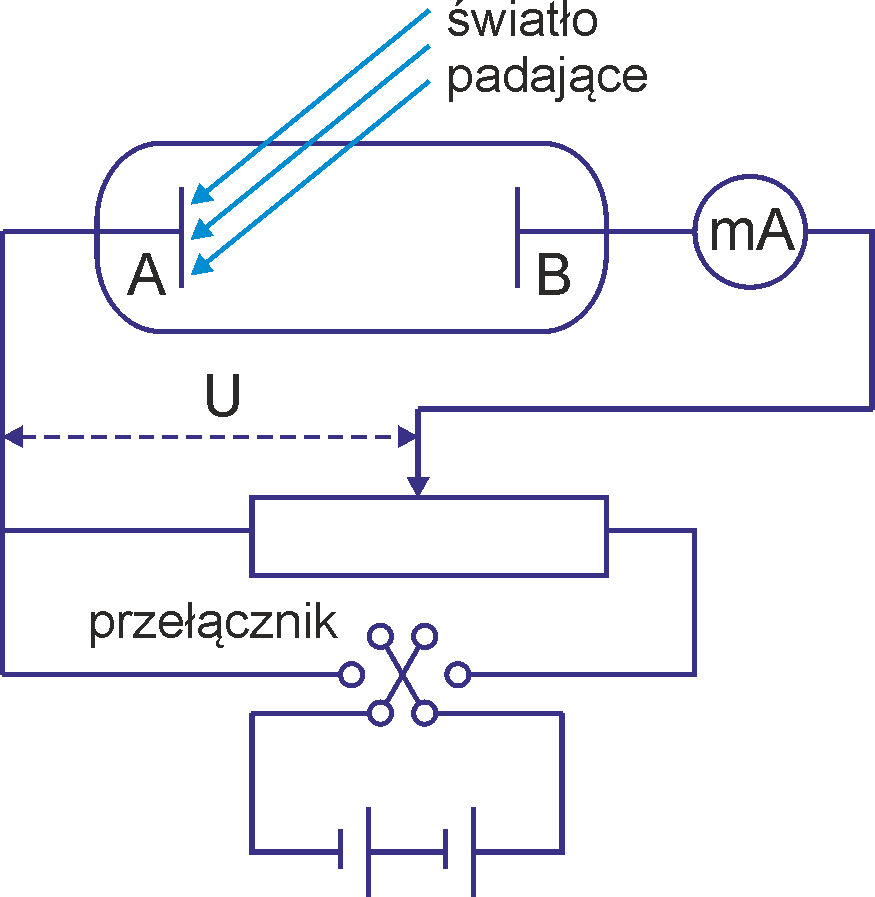
\includegraphics[width=0.5\textwidth]{efekt-fotoelektryczny}
    \caption{Układ do obserwacji zjawiska fotoelektrycznego. \textit{Źródło: e-Fizyka, AGH}}
    \label{fig:efekt-fotoelektryczny}
\end{figure}

W 1900 roku doświadczenia Lenarda wykazały, że energia elektronów zależy od częstotliwości światła, a nie jego intensywności.
Einstein sformułował wzór efektu fotoelektrycznego
\begin{equation*}
    \frac{1}{2} m v_{\max}^2 = h\nu - W,
\end{equation*}
gdzie $W$ to funkcja pracy metalu (zależna od rodzaju metalu).

\subsection{Widma atomowe i model Bohra}
Newton (1660) badał rozszczepienie światła. Melvill (1755) odkrył, że różne pierwiastki mają charakterystyczne linie widmowe. Kirchhoff (1855) zauważył, że widmo zależy od typu atomu i istnieją zarówno widma emisyjne, jak i absorpcyjne.

Balmer (1885) podał wzór:
\begin{equation*}
    \lambda = C \cdot \frac{n^2}{n^2 - 4}.
\end{equation*}

Rydberg sformułował bardziej ogólny wzór:
\begin{equation*}
    \tilde{\nu} = R_H \left( \frac{1}{2^2} - \frac{1}{n^2} \right).
\end{equation*}

\section{Funkcja falowa}

\subsection{Eksperyment z dwoma szczelinami}

Wobrażmy sobie ścianę z dwoma wąskimi otworami oraz drugą równoległą ścianę za nią, która nie ma żadnych otworów.
Teraz wyobraźmy sobie, że osoba strzela kulami we wszystkich kierunkach. Większość kul zatrzymuje się na pierwszej ścianie,
lecz część kul przechodzi przez otwory i trafia na drugą ścianę.
Jakiego obrazu spodziewamy się na drugiej ścianie? Spodziewamy się dwóch kropek, w miejscach odpowiadających otworom na pierwszej ścianie. To też obserwujemy.

\begin{figure}[H]
    \centering
    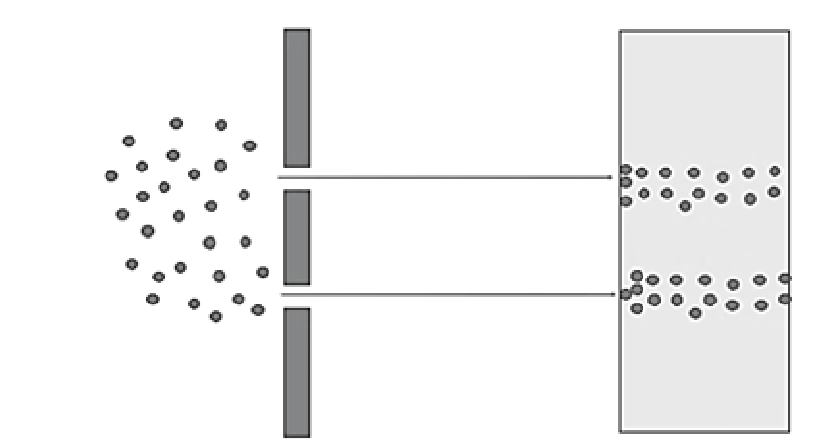
\includegraphics[width=0.5\textwidth]{szczeliny}
    \caption{Eksperyment z dwoma szczelinami. \textit{Źródło: Ranjbar, Vahid. (2023)}}
    \label{fig:szczeliny}
\end{figure}

\subsection{Eksperyment ze światłem}
W roku 1801 Thomas Young przeprowadził podobny eksperyment, ale przepuszczając przez szczeliny światło.
Przez dwie szczeliny przechodziła tak zwana fala płaska, poruszająca się w kierunku ekranu.
W sensie optyki klasycznej albo termodynamiki klasycznej, możemy powiedzieć, że przykładowo światło słoneczne jest taką falą płaską.
Ta fala płaska przechodzi przez szczeliny, a następnie dalej jako fala płaska przemieszcza się w kierunku oddalonego ekranu.

Co zobaczymy na ekranie? Na ekranie zobaczymy coś niespodziewanego - będzie to obraz interferencyjny.
\begin{figure}[H]
    \centering
    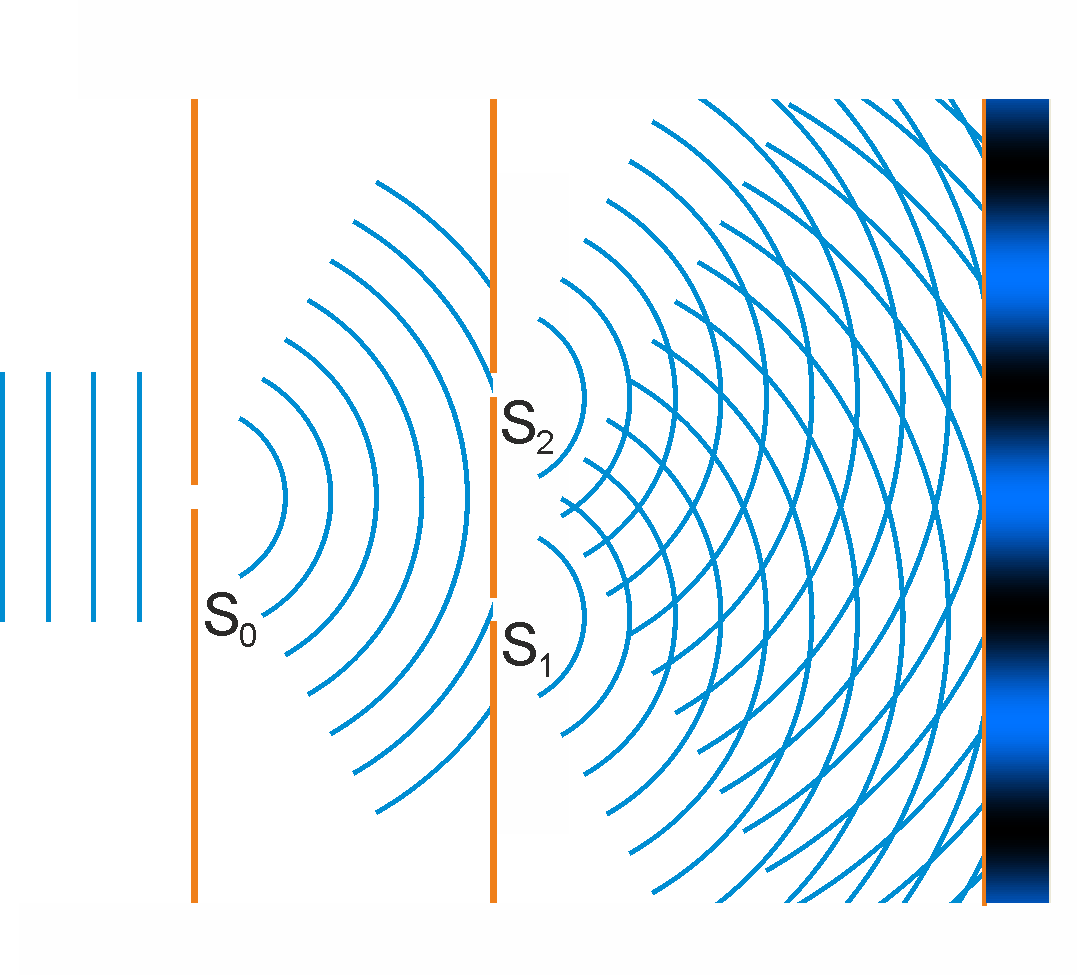
\includegraphics[width=0.5\textwidth]{szczeliny-fale}
    \caption{Eksperyment z dwoma szczelinami. \textit{Źródło: e-Fizyka, AGH}}
    \label{fig:szczeliny-fale}
\end{figure}

Zastanówmy się, w jaki sposób można opisać intensywności światła ukazujące się na ekranie.

Zacznijmy od amplitudy fali (amplitudy światła) - jest to wektor zależny od położenia w przestrzeni oraz czasu:
\begin{equation*}
    A(\bar{r}, t)
\end{equation*}
Intensnywność światła $I$ można zapisać jako kwadrat amplitudy niezależnej od modułu:
\begin{equation*}
    I = |A|^2
\end{equation*}
Następnie pojawia się tak zwana zasada superpozycji. Aby obliczyć amplitudę całkowitą, musimy zsumować amplitudy fal pochodzących z obu szczelin (z obu źródeł):
\begin{equation*}
    \bar{A}(\bar{r}, t) = \bar{A}_1(\bar{r}, t) + \bar{A}_2(\bar{r}, t)
\end{equation*}

Intensywność całkowita będzie przybierać następującą postać:
\begin{equation*}
    I = |A_1|^2 + |A_2|^2 + A_1 A_2^* + A_1^* A_2
\end{equation*}

Człon $A_1 A_2^* + A_1^* A_2$ jest odpowiedzialny za interferencję. Obraz widoczny na ekranie jest spowodowany superpozycją fal pochodzących z obu szczelin.

\subsection{Proste zagadnienie}

Rozważmy najprostsze zagadnienie. W tym zagadnieniu podkreślamy, że odległość między szczelinami $d$ jest mała (dużo mniejsza niż odległość do ekranu $D$).
Na ekranie zaznaczamy pewien punkt $x$ oraz zaznaczamy odległości punktu $x$ od szczelin. Odległość $x$ od szczeliny $1$ wynosi $r_1$, a odległość $x$
od szczeliny $2$ wynosi $r_2$.

\begin{figure}[H]
    \centering
    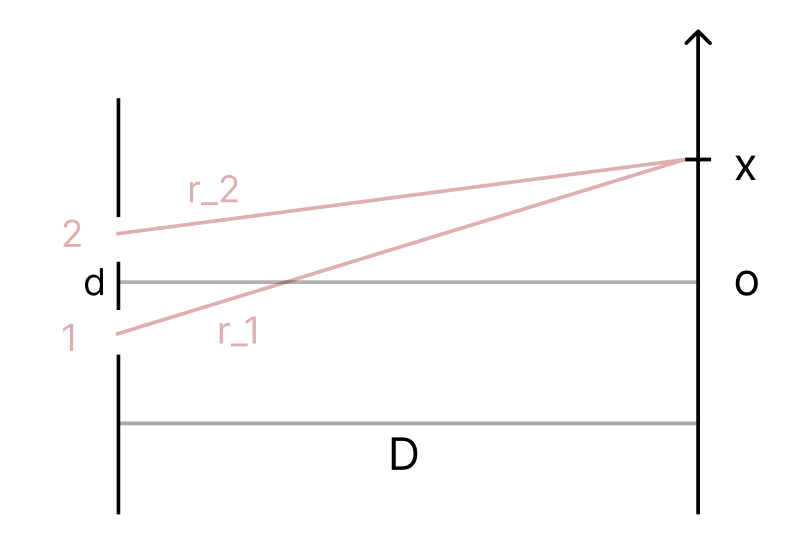
\includegraphics[width=0.5\textwidth]{prosty-eksperyment}
    \caption{Prosty eksperyment.}
    \label{fig:prosty-eksperyment}
\end{figure}

Rozważamy proste fale monochromatyczne, to znaczy amplitudy dla nich mają następującą postać:
\begin{equation*}
    A_1 = a_1 \exp[i(\omega t - \bar{k} \bar{r}_1 + \delta_1)]
\end{equation*}
\begin{equation*}
    A_2 = a_2 \exp[i(\omega t - \bar{k} \bar{r}_2 + \delta_2)]
\end{equation*}

Ponieważ mamy jedno źródło światła, możemy przyjąć, że $a_1 = a_2 = a$ i $\delta_1 = \delta_2 = 0$. 
Symbol $k$ oznacza wektor falowy, który ma kierunek fali. Zapisujemy go jako:
\begin{equation*}
    k = \frac{2\pi}{\lambda}
\end{equation*}
Wersor kierunku fali zapisujemy jako:
\begin{equation*}
    \frac{\bar{k}}{|k|}
\end{equation*}
Przechodzimy do geometrii. Chcemy zrozumieć, jaka będzie intensywność w punkcie $x$ na ekranie.

Wektory $\bar{k}_1$ i $\bar{k}_2$ będą równoległe do siebie, zatem możemy zapisać: $\bar{k}_1 = \bar{k}_2$.


Wyznaczamy $r_1^2$ i $r_2^2$:
\begin{equation*}
    r_1^2 = D^2 + \left(x + \frac{d}{2} \right)^2
\end{equation*}
\begin{equation*}
    r_2^2 = D^2 + \left(x - \frac{d}{2} \right)^2
\end{equation*}
Stąd:
\begin{equation*}
    r_1^2 - r_2^2 = 2xd
\end{equation*}
Ponieważ $r_1$ i $r_2$ są bardzo duże, a różnica między nimi jest mała, możemy zapisać:
\begin{equation*}
    r_1 - r_2 \approx \frac{xd}{D}
\end{equation*}
Intensywność końcowa:
\begin{align*}
    I &= \left(a\cdot e^{i\omega t}\right)^2 \cdot \left[e^{-ikr_1}+e^{-ikr_2}\right]^2 \\
    &= 2 a^2 \left(\cos{\left(kr_1-kr_2\right)}+1\right) \\
    &= 2 a^2 \left(1 + \cos{\left(k(r_1-r_2)\right)}\right) \\
    &= 2 a^2 \left(1 + \cos{\left(\frac{2\pi}{\lambda}\cdot\frac{xd}{D}\right)}\right) = I(x)
\end{align*}

Pytanie - dla jakich $x$ będzie maksymalna intensywność?
Aby znaleźć maksimum, obliczamy pochodną $I(x)$ i przyrównujemy do zera - wartość w zerze będzie albo maksimum, albo minimum.
Chcemy zatem, aby argument cosinusa przyjmował wartość $1$. Będzie to dla $2k\pi$, $k=0,1,2,3,\ldots$. Przyrównując:
\begin{equation*}
    \frac{2\pi}{\lambda} \frac{xd}{D} = 2k\pi
\end{equation*}
Rozwiązując dla $x$ otrzymujemy:
\begin{equation*}
    x_{max} = k \frac{\lambda D}{d}
\end{equation*}
W ten sposób możemy wytłumaczyć obraz interferencyjny - pojawiają się punkty o maksymalnej intensywności
rozłożone wzdłuż osi $x$, a odległość między kolejnymi punktami wynosi $\frac{\lambda D}{d}$.

\section{Stany kwantowe}

\subsection{Eksperyment S-G w interpretacji Feynmana}

Zawartość tego wykładu pochodzi z książki  "'\textit{Feymana wykłady z fizyki} "'. Feyman prowadził te wykłady na początku lat 60 i w głównej mierze zebrały uwagę profesorów gdyż były zbyt ciężkie dla studentów. Przerobimy to w taki sposób, aby to było jasne.
Wprowadźmy oznaczenia. 

\begin{minipage}{0.6 \textwidth}
	\begin{figure}[H]
		\centering
		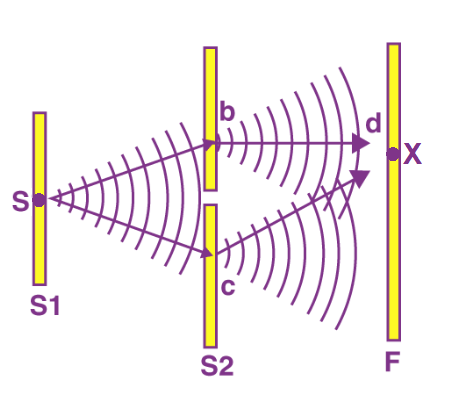
\includegraphics[width=0.5\textwidth]{eksperymentszczelinami}
		\caption{Eksperyment z dwoma szczelinami. \newline \textit{Źródło: Byju's}}
		\label{fig:szczeliny2}
	\end{figure}
\end{minipage}
\begin{minipage}{0.35 \textwidth}
	Prawdopodobieństwo, że elektron ze stanu S przejdzie do stanu X \newline [Stan $X$] $\leftarrow$ [Stan $S$] = $\vert\langle X\vert S\rangle\vert^2$ będziemy nazywać amplitudą.
\end{minipage}

Amplitudę ze stanu $S$ do stanu $X$ możemy w tym przypadku zapisać dwojako, w postaci $\langle X\vert1\rangle, \langle 1\vert S\rangle$ jako przejścia ze stanu $S$ do stanu $1$ a następnie ze stanu $1$ do stanu $X$, oraz analogicznie w postaci $\langle X\vert2\rangle , \langle 2\vert S\rangle$. Przepiszemy korzystając z tych oznaczeń zasadę superpozycji. Jeżeli chcemy przejść ze stanu $S$ do stanu $X$ to będziemy to zapisywać jako sumę amplitud $\langle X\vert S\rangle = \langle X\vert1\rangle\langle 1\vert S\rangle + \langle X\vert2\rangle \langle 2\vert S\rangle$. Jeżeli chcemy zapisać prawdopodobieństwo to musimy obliczyć z tego moduł do kwadratu i obliczyć to wszystko w liczbach zespolonych $\vert\langle X\vert S\rangle \vert^2 = \vert[...]\vert^2$. 
\textbf{Pytanie} co oznacza superpozycja? Jeżeli chcemy obliczyć amplitudę to jest to suma poszczególnych amplitud. Amplituda $S$ do $Z$ jest superpozycją przejścia przez szczeliny.
\subsection{Urządzenie S-G dla atomów ze spinem 1}
\begin{minipage}{0.2 \textwidth}
	\vspace{11pt}
	Spin oznaczamy
\end{minipage}
\begin{minipage}{0.11 \textwidth}
    \begingroup
    \hfuzz=1000pt
	\begin{equation*}
		X_{\beta} = 
		\begin{cases}
			+1 \\
			0 \hspace{20pt} \leftarrow \text{ trzy rodzaje kwantowe.} \\
			-1 \\
		\end{cases}
	\end{equation*}
    \endgroup
\end{minipage}
\begin{figure}[H]
	\centering
	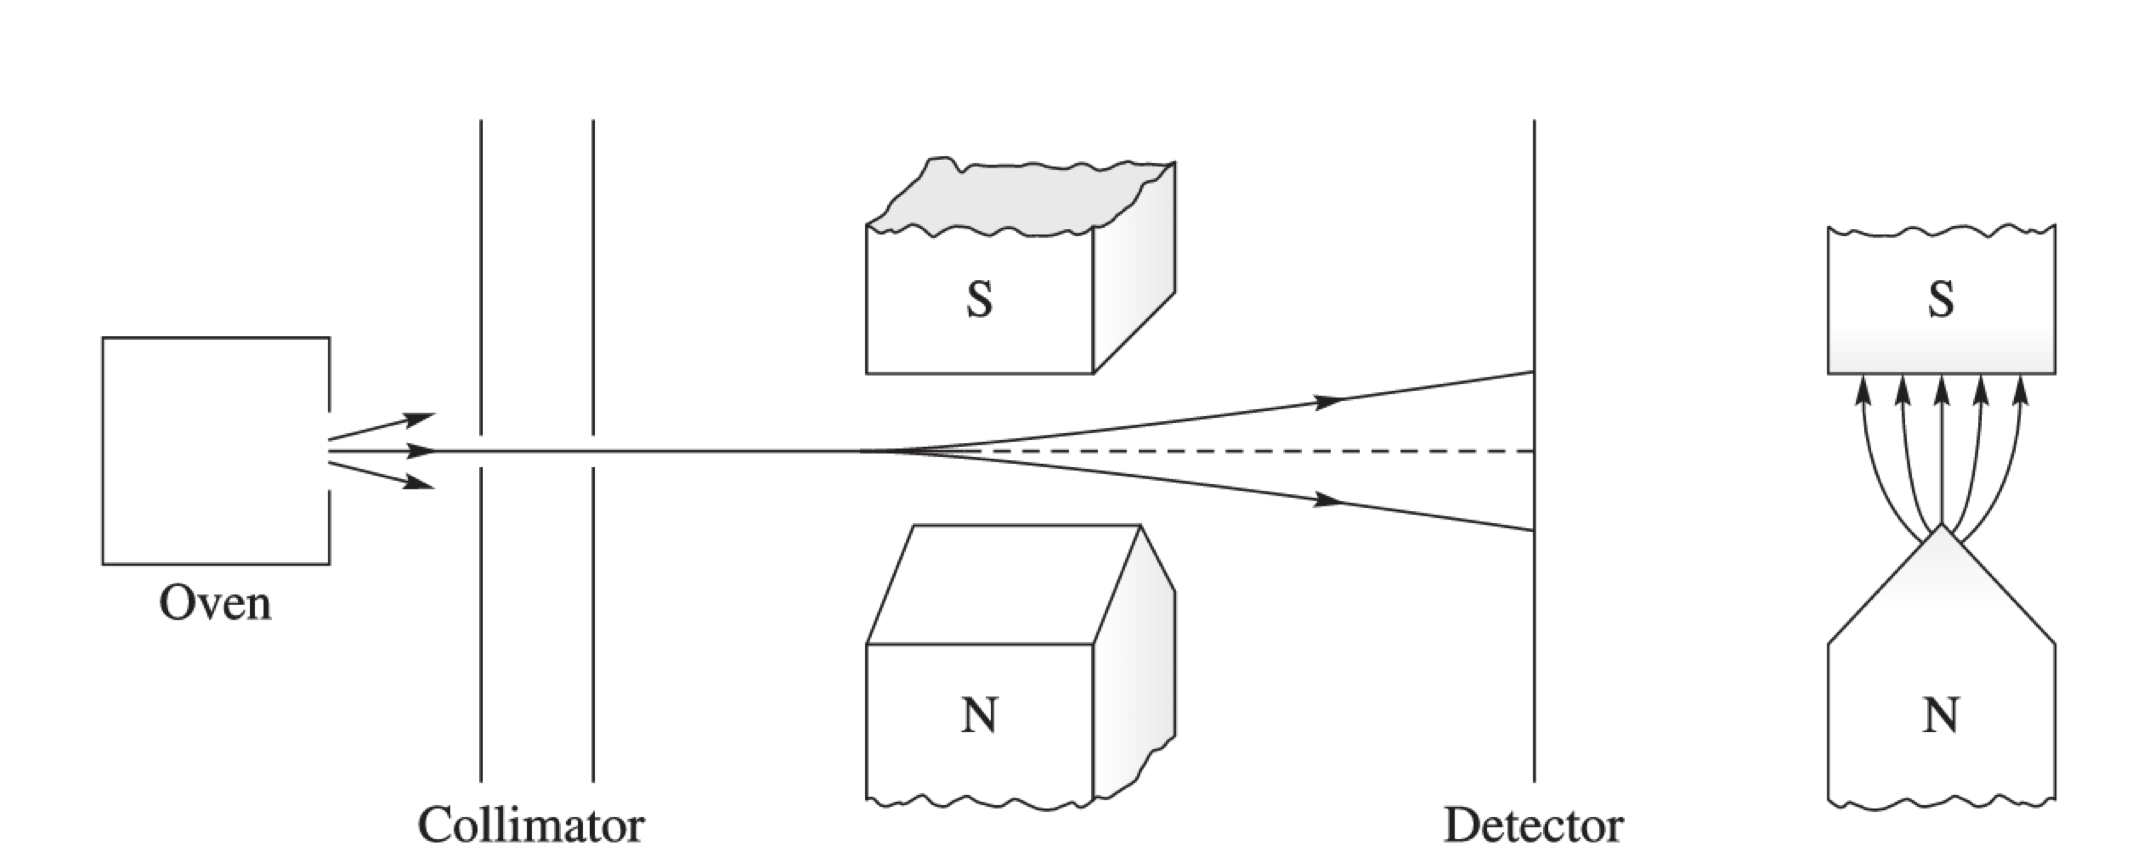
\includegraphics[width=0.6\textwidth]{urzadzeniesg}
	\caption{Urządzenie Sterna-Gerlacha. \textit{Źródło: PennState ESM}}
	\label{fig:urzSG}
\end{figure}
\begin{figure}[H]
	\centering
	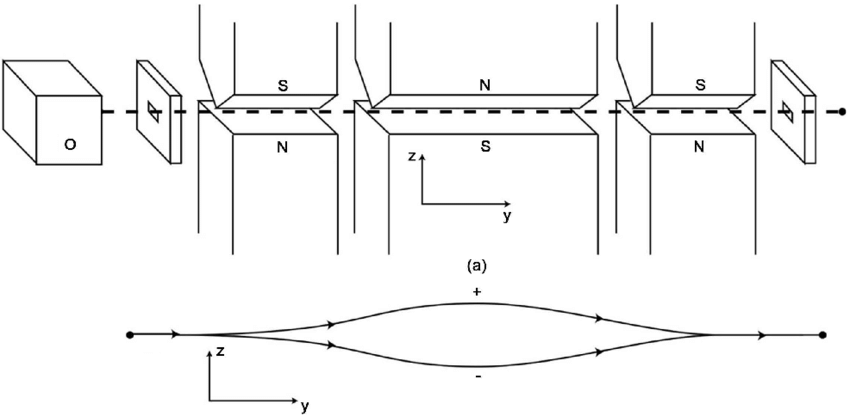
\includegraphics[width=0.8\textwidth]{urzadzeniesgmod.png}
	\caption{Modyfikacja urządzenia Sterna-Gerlacha. \textit{Źródło: ResearchGate}}
	\label{fig:urzSGmod}
\end{figure}
Dlaczego tak robimy? Ponieważ dzięki zmodyfikowaniu urządzenia S-G nasze atomy będą podążały jak na rysunku powyżej do jednego punktu. I to będzie nasze modyfikowane urządzenie S-G o którym dalej będziemy mówić. Następnie możemy rozważyć kolejny schemat. Możemy wstawić płytkę przez którą nie mogą przechodzić atomy, więc na końcu będziemy mieli tylko atomy nie zablokowane.

\begin{minipage}{0.5 \textwidth}
	\begin{figure}[H]
		\centering
		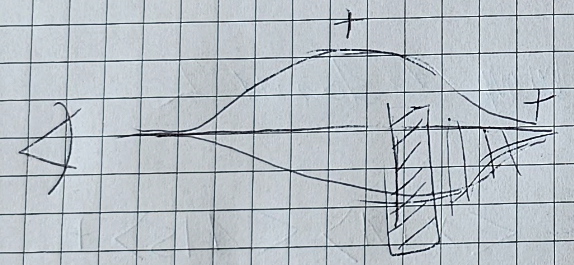
\includegraphics[width=0.8\textwidth]{urzadzeniesgblok}
		\caption{Zablokowane atomy poza  "'$+$ "'}
		\label{fig:urzSGblok}
	\end{figure}
\end{minipage}
\begin{minipage}{0.05 \textwidth}
	\vspace{-20pt}
	\begin{equation*}
		\hspace{-30pt}
		\left\{\begin{array}{lr}
			+ \\
			0 \hspace{3pt} \vert \\
			- \vert
		\end{array}\right\}
	\end{equation*}
\end{minipage}
\begin{minipage}{0.45 \textwidth}
	Będziemy podpisywać modyfikacje z zablokowanymi  "'$0$ "' oraz  "'$-$ "' jako  "'$+S$ "', analogicznie  "'$0S$ "' oraz  "'$-S$ "'
\end{minipage}


\begin{minipage}{0.6 \textwidth}
	\begin{figure}[H]
		\centering
		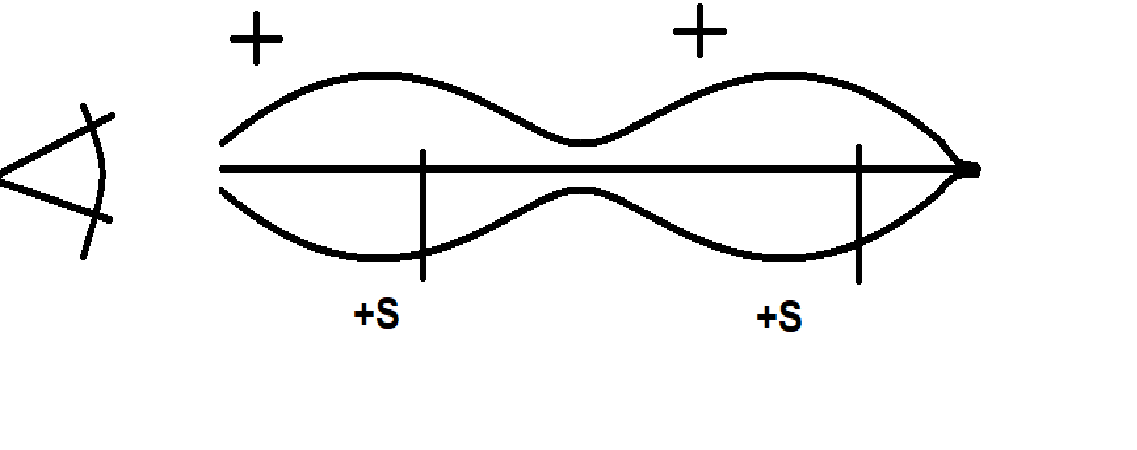
\includegraphics[width=0.6\textwidth]{urzsgblok2}
		\caption{Zablokowane atomy poza  "'$+$ "' dwa razy}
		\label{fig:urzSGblok2}
	\end{figure}
\end{minipage}
\begin{minipage}{0.5 \textwidth}
	\vspace{-40pt}
	$\langle +S \vert +S \rangle = 1$, dlatego że wszystkie atomy przejdą najpierw górnym, a potem będą tylko i wyłącznie dostępne atomy z plusem, więc wszystkie atomy znowu przejdą, więc zawsze wychodzi $1$. Jest to postulat.
\end{minipage}


\begin{minipage}{0.6 \textwidth}
	\begin{figure}[H]
		\centering
		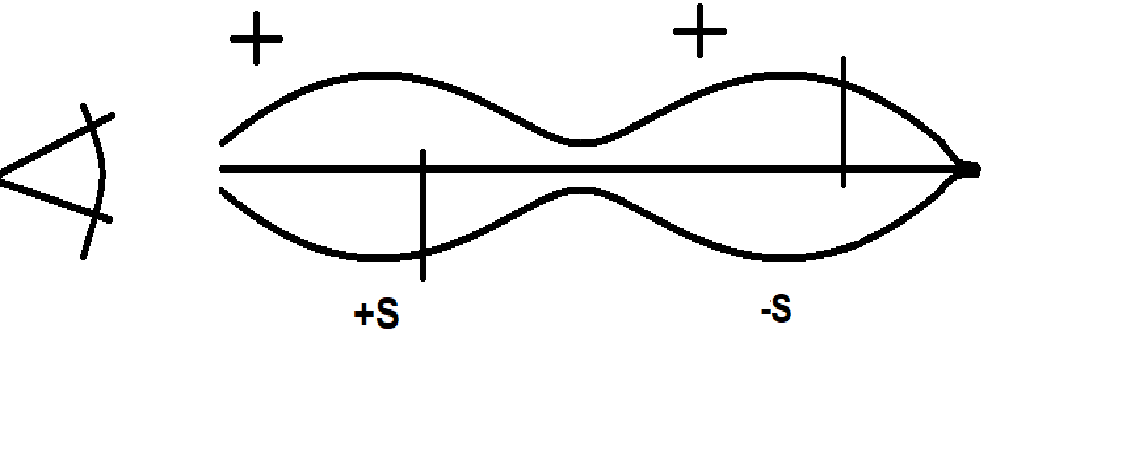
\includegraphics[width=0.6\textwidth]{urzsgblok3}
		\caption{Zablokowane atomy raz poza  "'$+$ "' i raz poza  "'$-$ "'}
		\label{fig:urzSGblok3}
	\end{figure}
\end{minipage}
\begin{minipage}{0.5 \textwidth}
	\vspace{-40pt}
	$\langle -S \vert +S \rangle = 0$
\end{minipage}
\newpage
Możemy w taki sposób wymienić różne stany początkowe i końcowe i możemy stworzyć tabelę
\begin{table}[ht]
	\centering
	\begin{tabular}[t]{c|c|c|c}
		& $+S$ & $0S$ & $-S$\\
		\hline
		$+S$ & $1$ & $0$ & $0$ \\
		\hline
		$0S$ & $0$ & $1$ & $0$ \\
		\hline
		$-S$ & $0$ & $0$ & $1$ \\
	\end{tabular}
	\label{tab:stany}
\end{table}

Następnie rozważmy sytuacje gdzie mamy  "'pokręcone "' urządzenie S-G. Niech pierwsze urządzenie będzie się nazywało urządzeniem "'$S$"' a drugie urządzeniem "'$T$"'

\begin{figure}[H]
	\centering
	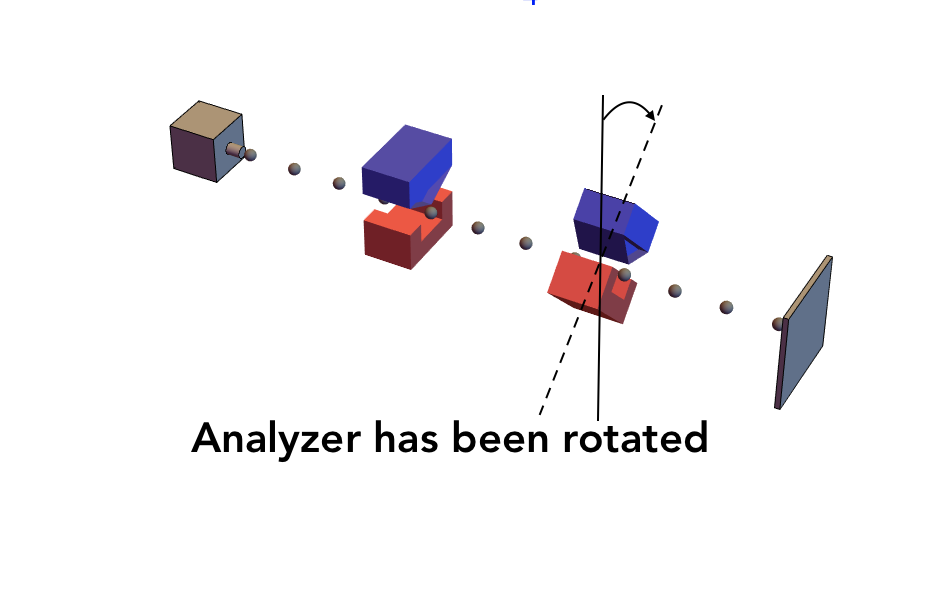
\includegraphics[width=0.8\textwidth]{SGArot}
	\caption{Obrócone urządzenie S-G, \textit{Źródło: Deepnote}}
	\label{fig:SGArot}
\end{figure}

Jeżeli mamy na początku stan "'$+S$ "'  a następnie przechodzimy przez urządzenie ze stanem "'$-T$ "' to co będziemy mieli? 


\begin{equation*}
	\left\{\begin{array}{lr}
		+ \\
		0 \hspace{3pt} \vert \\
		- \vert
	\end{array}\right\} 
	\left\{\begin{array}{lr}
		+ \vert \\
		0 \hspace{3pt} \vert \\
		- 
	\end{array}\right\}
	\neq 0 \text{,} \hspace{10pt}  \langle-T \vert +S\rangle \neq 0
\end{equation*}
Jeżeli chcemy obliczyć prawdopodobieństwo przejścia ze stanu "'$+S$ "' do stanu "'$+T$ "' to możemy to obliczyć następująco
\begin{equation*}
	\left| \langle\ +T\vert+S \rangle \right|^2 = \langle\ +T\vert+S \rangle \langle\ +T\vert+S \rangle^*
\end{equation*}
Gdy prowadzimy kilka doświadczeń w których będziemy mieli początek w "' $+S$ "' a następnie przejdziemy przez urządzenia "'$+T$ "' i  "'$0T$ "' oraz "'$0T$ "', to prawdopodobieństwo że cząstka przejdzie końcowo przez którekolwiek z urządzeń "'$T$ "' jest jedynką.

\begin{equation*}
	\langle\ +T\vert+S \rangle \langle\ +T\vert+S \rangle^* + \langle\ 0T\vert+S \rangle \langle\ 0T\vert+S \rangle^* +\langle\ -T\vert+S \rangle \langle\ -T\vert+S \rangle^* =1
\end{equation*}
Następnie rozważmy schemat eksperymentu gdzie najpierw mamy urządzenie "' $0S$ "', następnie "' $0T$ "' a końcowo "' $+S$ "'. Wtedy amplituda $\langle\ +S\vert0T \rangle \langle\ 0T\vert0S \rangle^*$ będzie następująca
\begin{equation*}
	\frac{p_2}{p_1} = \frac{\left|\langle\ +S\vert0T \rangle \langle\ 0T\vert0S \rangle\right|^2}{\left|\langle\ 0S\vert0T \rangle \langle\ 0T\vert0S \rangle\right|^2} = \frac{\left|\langle\ +S\vert0T \rangle\right|^2}{\left|\langle\ 0S\vert0T \rangle\right|^2}
\end{equation*}
Rozważmy trzy schematy eksperymentu gdzie $N$ cząstek będzie przechodzić z urządzenia "' $S$ "' do urządzenia "' $T$ "' i znowu do "' $S$ "'.
\begin{equation*}
	\hspace{-50pt} (1)
	\left\{\begin{array}{lr}
		+ \\
		0 \hspace{3pt} \vert \\
		- \vert
	\end{array}\right\} 
	\xrightarrow[N]{}
	\left\{\begin{array}{lr}
		+  \\
		0  \\
		- 
	\end{array}\right\}
	\xrightarrow[N]{}
	\left\{\begin{array}{lr}
		+  \\
		0 \hspace{3pt} \vert \\
		- \vert
	\end{array}\right\}
	\xrightarrow[N]{} \text{To urządzenie nic nie zmienia}
\end{equation*}

\begin{equation*}
	\hspace{-140pt} (2)
	\left\{\begin{array}{lr}
		+ \\
		0 \hspace{3pt} \vert \\
		- \vert
	\end{array}\right\} 
	\xrightarrow[N]{}
	\left\{\begin{array}{lr}
		+  \\
		0  \\
		- 
	\end{array}\right\}
	\xrightarrow[N]{}
	\left\{\begin{array}{lr}
		+ \vert \\
		0  \\
		- \vert
	\end{array}\right\}
	\xrightarrow[0]{} \text{Zero cząstek}
\end{equation*}

\begin{equation*} (3)
	\left\{\begin{array}{lr}
		+ \\
		0 \hspace{3pt} \vert \\
		- \vert
	\end{array}\right\} 
	\xrightarrow[N]{}
	\left\{\begin{array}{lr}
		+ \vert \\
		0 \hspace{3pt} \vert \\
		- 
	\end{array}\right\}
	\xrightarrow[N]{}
	\left\{\begin{array}{lr}
		+ \vert \\
		0  \\
		- \vert
	\end{array}\right\}
	\xrightarrow[\beta\alpha N]{\alpha \leq 1, \beta \leq 1} \text{Tu przechodzi tylko część cząstek}
\end{equation*}
W przypadku eksperymentu $(3)$, urządzenie "' $T$ "' jest bardziej restrykcyjne niż w przypadku eksperymentu $(2)$, jednak mimo tego końcowo przechodzi niezerowa ilość cząstek. To jest przykład zupełnie kwantowy.
Można to zrozumieć analogicznie w kontekście wektorów, przy standardowym rzutowaniu najpierw na oś $OY$ a następnie na $OX$ zawsze kończymy w zerze, jednak gdybyśmy mieli dodatkowe osie $OY'$ oraz $OX'$ i rzutowali po kolei $OY \rightarrow OY' \rightarrow OX$ to pomimo nałożenia dodatkowego restrykcyjnego rzutowania otrzymujemy wynik niezerowy.
Ze schematu drugiego widzimy
\begin{equation*}
	a = 0 = \left|\langle\ 0S \vert +T \rangle \right| \left|\langle\ +T \vert +S \rangle \right| + 
	\left|\langle\ 0S \vert 0T \rangle \right| \left|\langle\ 0T \vert +S \rangle \right| + 
	\left|\langle\ 0S \vert -T \rangle \right| \left|\langle\ -T \vert +S \rangle \right|
\end{equation*}
Amplitudy mamy interferencyjne i w rezultacie mamy 0. Ze schematu pierwszego natomiast
\begin{equation*}
	a = 1 = \left|\langle\ +S \vert +T \rangle \right| \left|\langle\ +T \vert +S \rangle \right| + 
	\left|\langle\ +S \vert 0T \rangle \right| \left|\langle\ 0T \vert +S \rangle \right| + 
	\left|\langle\ +S \vert -T \rangle \right| \left|\langle\ -T \vert +S \rangle \right|
\end{equation*}
\subsection{Bazy}
Niech $\vert +T \rangle = \vert 1 \rangle$, $\vert 0T \rangle = \vert 2 \rangle$, $\vert -T \rangle = \vert 3 \rangle$. Wtedy możemy zapisać amplitudę $a$ jako sumę
\begin{equation*}
	a = \sum_{i = 1}^3 \langle\ +S \vert i \rangle \langle\ i \vert +S \rangle = 1 = \langle\ +S \vert +S \rangle
\end{equation*}
Dzięki temu możemy zapisać niezależnie od tego jakie mamy urządzenia. Dla schematu z urządzeniami $S$ oraz $R$ mamy
\begin{equation*}
	\left\{\begin{array}{lr}
		+ \\
		0 \hspace{3pt} \vert \\
		- \vert
	\end{array}\right\} 
	\left\{\begin{array}{lr}
		+ \\
		0 \hspace{3pt} \vert \\
		- \vert
	\end{array}\right\} 
	\iff a =  \langle\ +R \vert +S \rangle \langle\ = \sum_{i = 1}^3 \langle\ +R \vert i \rangle \langle\ i \vert +S \rangle
\end{equation*}
Zapiszmy $\vert +R \rangle = \vert \chi \rangle$, $\vert +S \rangle = \vert \phi \rangle$, i wtedy mamy zapis które wszędzie można spotkać w mechanice kwantowej
\begin{equation*}
	\langle\ \chi \vert \phi \rangle = \sum_{i} \langle\ \chi \vert i \rangle \langle\ i \vert \phi \rangle
\end{equation*}
Możemy z tego zapisać kilka reguł (pod warunkiem że $i \neq j$)
\begin{equation*}
	\begin{split}
		\langle\ i \vert i \rangle &= 1 \\
		\langle\ i \vert j \rangle &= 1
	\end{split}
\end{equation*}
Przepiszmy równanie które już wcześniej wyliczyliśmy w tym rozdziale.
\begin{equation*}
	\langle\ +T\vert+S \rangle \langle\ +T\vert+S \rangle^* + \langle\ 0T\vert+S \rangle \langle\ 0T\vert+S \rangle^* +\langle\ -T\vert+S \rangle \langle\ -T\vert+S \rangle^* =1.
\end{equation*}
Łącząc je z równaniem dające wynik amplitudy $a = 1$ dostajemy zależności
\begin{equation*}
	\begin{split}
		\langle\ +S \vert +T \rangle &= \langle\ +T \vert +S \rangle^* \\
		\langle\ +S \vert 0T \rangle &= \langle\ 0T \vert +S \rangle^* \\
		\langle\ +S \vert -T \rangle &= \langle\ -T \vert +S \rangle^* 
	\end{split}
\end{equation*}
Daje nam to kolejną regułę
\begin{equation*}
	\langle\ \chi \vert \phi \rangle = \langle\ \phi \vert \chi \rangle^*
\end{equation*}
\subsection{Operatory}
Amplitudę że przejdziemy ze stanu $+S$ do $0R$ możemy zapisać jako
\begin{equation*}
	a = \langle\ 0R \vert \dots \rangle \langle\ \dots \vert \dots \rangle \dots \langle\ \dots \vert \dots \rangle \langle\ \dots \vert +S \rangle  = \langle\ 0R \vert A \vert +S \rangle 
\end{equation*}
gdzie $A$ to są różne operacje związane ze zbiorem urządzeń. Przez $\hat{A}$ będziemy oznaczać operator generalny.
Możemy też zapisać macierz operatora $\hat{A}$. Niech $\vert +S \rangle$, $\vert 0S \rangle$, $\vert -S \rangle$ będą stanami naszej bazy. Wtedy mamy
\begin{table}[ht]
	\centering
	\begin{tabular}[t]{c|c|c|c}
		& $+$ & $0$ & $-$\\
		\hline
		$+$ & $\langle\ + \vert \hat{A} \vert + \rangle $ & $\langle\ + \vert \hat{A} \vert 0 \rangle $ & $\langle\ + \vert \hat{A} \vert - \rangle $ \\
		\hline
		$0$ & $\langle\ 0 \vert \hat{A} \vert + \rangle $ & $\langle\ 0 \vert \hat{A} \vert 0 \rangle $ & $\langle\ 0 \vert \hat{A} \vert - \rangle $ \\
		\hline
		$-$ & $\langle\ - \vert \hat{A} \vert + \rangle $ & $\langle\ - \vert \hat{A} \vert 0 \rangle $ & $\langle\ - \vert \hat{A} \vert - \rangle $ \\
	\end{tabular}
	\label{tab:macierzoperatora}
\end{table}

Powyższe nazywamy macierzą operatora $\hat{A}$ w bazie takiej jak wyżej podanej. Dajemy też czapkę nad operatorem aby zawsze było wiadomo że chodzi nam o operator, ale nie zawsze trzeba to pisać. Operator nigdy nie jest zależny od bazy ale macierz operatora zawsze jest w jakiejś bazie.
Następnie wyprowadźmy parę własności.
\begin{equation*}
	\left\{\begin{array}{lr}
		+ \\
		0  \\
		- 
	\end{array}\right\}_{S} 
	\left\{\begin{array}{lr}
		+ \\
		0 \\
		- 
	\end{array}\right\}_{T_i}
	\hat{A}
	\left\{\begin{array}{lr}
		+ \\
		0  \\
		- 
	\end{array}\right\}_{T_j} 
	\left\{\begin{array}{lr}
		+ \vert \\
		0 \\
		- \vert
	\end{array}\right\}_{R}
	=
	\left\{\begin{array}{lr}
		+ \\
		0  \\
		- 
	\end{array}\right\}_{S} 
	\hat{A}
	\left\{\begin{array}{lr}
		+ \vert \\
		0 \\
		- \vert
	\end{array}\right\}_{R}
\end{equation*}
Możemy powiedzieć że weźmiemy bazę tego urządzenia $T$ i wtedy możemy to zapisać inaczej jako

\begin{equation*}
	\sum_{ij} \langle\ 0R \vert j \rangle \langle\ j \vert A \vert i \rangle \langle\ i \vert +S \rangle = \langle\ OR \vert A \vert +S \rangle
\end{equation*}
Inaczej możemy zapisać, uogólniając tą regułę, że 
\begin{equation*}
	\langle\ \chi \vert A \vert \phi \rangle = \sum_{ij} \langle\ \chi \vert j \rangle \langle\ j \vert A \vert i \rangle \langle\ i \vert \phi \rangle
\end{equation*}
Niech urządzenie $C$ to urządzenie $B$ które stoi tuż po urządzeniu $A$.
\begin{equation*}
	\{C\} = \{A\} \{B\} = \{A\} \left\{\begin{array}{lr}
		+ \\
		0 \\
		- 
	\end{array}\right\}_{T} \{B\}
\end{equation*}
Przez to możemy zapisać
\begin{equation*}
	\langle\ j \vert C \vert i \rangle = \sum_{ij} \langle\ j \vert B \vert k \rangle \langle\ k \vert A \vert i \rangle
\end{equation*}
A także zapisać to jak mnożenie macierzowe
\begin{equation*}
	\hat{C} = \hat{A} \cdot \hat{B} \rightarrow C = A \cdot B
\end{equation*}
\subsection{Przekształcenia bazy}
Powiedzmy że $\hat{A}$ - operator. Mamy też dwie dowolne ortonormalne bazy $\{1\}$ oraz $\{2\}$. Pytanie jest takie: powiedzmy że mamy operator $\langle\ i_1 \vert \hat{A} \vert j_1 \rangle$. W jaki sposób będą wyglądały elementy macierzowe operatora $\hat{A}$ w bazie $\{2\}$? Do tego potrzebujemy przekształcenia bazy.
\begin{equation*}
	\vert i_2 \rangle = \sum_{j_1} D_{i_2 j_1} \vert j_1 \rangle 
\end{equation*}
Wprowadźmy też tutaj nazewnictwo $\langle j \vert$ - stan "bra", $\vert i \rangle$ - stan "kiet".
Jeżeli ${\vert i \rangle}$ - baza, a $\vert \phi \rangle$ - stan, i jeżeli z tych mamy amplitudy $\langle i \vert \phi \rangle = C_i$, $\langle j \vert \phi \rangle = C_j$, to wtedy możemy powiedzieć że
\begin{equation*}
	\vert \phi \rangle = \sum_{i} C_i \vert i \rangle 
\end{equation*}
Gdzie $C_i$ to amplitudy lub współczynniki. Możemy też pisać
\begin{equation*}
	\vert \chi \rangle = \begin{pmatrix} c_1 \\ c_2 \\ c_3 \end{pmatrix} = c_1 \vert 1 \rangle + c_2 \vert 2 \rangle + c_3 \vert 3 \rangle 
\end{equation*}
W takiej sytuacji piszemy że jakieś $\chi$ jest wektorem, jakimś rozłożeniem w bazie przestrzeni którą mamy. 
Niech też wektor "kiet" będzie 
\begin{equation*}
	\vert \chi \rangle = \sum_i \vert i \rangle D_i.
\end{equation*}
Wtedy wektor "bra" możemy zapisać następująco
\begin{equation*}
	\langle \chi \vert = \sum_j \rangle D_i^* \langle i \vert.
\end{equation*}
Dlaczego tak piszemy? Zobaczmy że dzięki naszemu zapisowi mamy poniższe
\begin{equation*}
	\langle \chi \vert \chi \rangle =  1 = \sum_{ij} \langle i \vert j \rangle D_i^* D_j.
\end{equation*}
Wtedy jeżeli mamy policzyć amplitudę $\langle \chi \vert \phi \rangle$ mamy
\begin{equation*}
	\langle \chi \vert \chi \rangle = \sum_{ij} D_j^* \langle j \vert i \rangle C_i = \sum_i D_i^* C_i
\end{equation*}
I w taki sposób będziemy obliczać powyższą amplitudę z przekształceniem bazy. Zapiszmy też
\begin{equation*}
	\langle\ i_2 \vert A \vert j_2 \rangle = \left(\sum_k D_{il}^* \langle l_1 \vert  \right) A \left(\sum_k D_{jk} \vert k_1 \rangle \right) = \sum_{lk} D_{il}^* D_{jk} \langle l_1 \vert A \vert k_1 \rangle
\end{equation*}
Nie wszystkie bazy są takie same, każde zagadnienie potrzebuje odpowiedniej (wygodnej) bazy i będziemy się tego uczyć.
\subsection{Równanie Schrödingera}
Czas wpływa na ewolucje dowolnego układu kwantowego. $U(t_2, t_1)$ - operator ewolucji.
\begin{equation*}
	\langle \chi \vert \hat{U}(t_2, t_1)\vert \phi \rangle - \text{amplituda}, \vert \phi \rangle \xrightarrow{t_1 \rightarrow t_2} \vert \chi \rangle
\end{equation*}
\begin{equation*}
	\langle i \vert \hat{U}(t_2, t_1)\vert j \rangle, \text{ gdzie $t_2$ - czas końcowy, $t_1$ - czas początkowy}
\end{equation*}
Mówimy, że operator ewolucji posiada własność
\begin{equation*}
	U(t_3, t_1) = U(t_3,t_2)U(t_2,t_1) \leftarrow \text{ postulat}
\end{equation*}
Dla $\delta t$ małego czasu możemy wypisywać, że stan układu w czasie
\begin{equation*}
	\vert \psi (t + \Delta t) \rangle = U(t+\Delta t, t\vert \psi(t) \rangle )
\end{equation*}
Możemy obliczyć współczynniki amplitudy dla stanu bazowego i
\begin{equation*}
	C_i(t+\Delta t) \leftarrow \langle i \vert \psi(t + \Delta t) \rangle = \langle i \vert U(t + \Delta t, t) \vert \psi(t)\rangle = \sum_j \langle i \vert U(t + \Delta t, t) \vert j \rangle \langle j \vert \psi(t) \rangle \rightarrow C_j(t)
\end{equation*}
\begin{equation*}
	C_j(t+\Delta t) = \sum_j U_{ij}(t + \Delta t, t) C_j(t)
\end{equation*}
Mamy też postulat
\begin{equation*}
	U_{ij}(t + \Delta t, t) = \delta_{ij} - \frac{i}{\hbar}H_{ij}(t)\Delta t
\end{equation*}
Gdzie $\frac{i}{\hbar}H_{ij}(t)$ jest wygodnym elementem macierzowym i korzystnym później. Gdy mamy operator $U_{ij}(t, t)$ to nic się nie zmienia [trywialne]. Wykonajmy teraz kilka przekształceń
\begin{equation*}
	\begin{split}
		C_j(t + \Delta t) &= \sum_j (\delta_{ij} - \frac{i}{\hbar}H_{ij}(t)\Delta t)C_J(t)\\
		C_j(t + \Delta t) &= C_j(t) - \frac{i}{\hbar}\Delta t \sum_j H_{ij} H(t) C_j(t) \\
		\frac{C_j(t + \Delta t) - C_j(t)}{\Delta t} &= - \frac{i}{\hbar} \sum_j H_{ij}(t) C_j(t)
	\end{split}
\end{equation*}
Korzystając teraz z zapisu $\dot{c}_i(t)$ - pochodna po czasie, zapiszmy
\begin{equation*}
	i\hbar \dot{c}_i(t) = \sum_j H_{ij}(t) C_j(t)
\end{equation*}
Niech także
\begin{equation*}
	\overrightarrow{c}(t) = \begin{pmatrix} c_1(t) \\ c_2(t) \\ \vdots \end{pmatrix}
\end{equation*}
Wtedy możemy zapisać
\begin{equation*}
	i\hbar \overrightarrow{c}(t) =  \hat{H}(t) \hat{C}(t)
\end{equation*}
\textbf{Pytanie} czy skoro H jest zależne od czasu tutaj, to później też takie będzie czy raczej stałe? To będzie zależeć od zagadnienia, ale łatwiej jest jak nie ma tej zależności.
Wiemy też że cząstka musi być w jakimś stanie, więc
\begin{equation*}
	\sum_i \vert C_i(t)\vert^2 = 1.
\end{equation*}

\textbf{Pytanie} skoro c jest niewiadoma to czy H jest znane? H jest znane (sztuka rozsądnego zgadywania) i takie aby równanie było poprawne.

\textbf{Pytanie} czy i to jest stan z bazy? Tak
\subsection{Przykład: Ewolucja atomu z 2 stanami w polu laserowym}
Powiedzmy, że mamy atom z 2 stanami (przybliżenie/uproszczenie). Wtedy mamy
\begin{equation*}
	i\hbar \begin{pmatrix} \dot{c}_1\\ \dot{c}_2 \end{pmatrix} = H \begin{pmatrix} \dot{c}_1\\ \dot{c}_2 \end{pmatrix} , \hspace{5pt} H = \hbar \begin{pmatrix} -\epsilon & \nu \\ \nu & \epsilon  \end{pmatrix}
\end{equation*}
\begin{equation*}
\epsilon, \nu \in \mathcal{R}, \hspace{5pt} c_1(0) = 1, \hspace{5pt} c_2(0) = 0
\end{equation*}
gdzie wartości przy drugim $\hbar$ to operator współdziałania

\textbf{Pytanie} wiemy że $\epsilon$ może byś dowolne, ale kiedy zmienia się $\nu$? Wpływa na to intensywność lasera i częstość lasera. Mając stany bazy i operator współdziałania możemy mieć $\nu$.

\textbf{Pytanie} czy w macierzy H po skosach mają być te same rzeczy? Tak.
Co jeżeli
\begin{equation*}
	H = \hbar \begin{pmatrix} E_1 & 0 \\ 0 & E_2  \end{pmatrix}?
\end{equation*}
\begin{equation*}
	\begin{cases}
		i \hbar \dot{c}_1 = E_1 C_1 \\
		i \hbar \dot{c}_2 = E_2 C_2
	\end{cases}
	\Rightarrow
	\begin{cases}
		C_1 = C_1(0) \exp{\frac{-iE_1t}{\hbar}} \\
		C_2 = \dots
	\end{cases}
\end{equation*}
\subsection{Funkcja falowa}
Elektron może być w stanach x1, x2, $\dots$.
 
\textbf{Pytanie} ile jest stanów, $\infty$ czy nie? Baza może być skończona lub nieskończona. Gdy baza jest nieskończona mamy przestrzeń Hilberta, tak jest w przyrodzie.
\begin{equation*}
	\begin{split}
		\vert \psi \rangle = \sum_i (i \vert X_i) = \int c(x) \vert x \rangle dx \\
		\psi(x) = C(x) - \text{ funkcja falowa} \\
		\langle x \vert \psi \rangle = c_x = c(x)
	\end{split}
\end{equation*}
Często będzie baza własna
\begin{equation*}
	\vert j \rangle = f_j(x) \leftarrow \text{ standardowy sposób opisania stanów i bazy}
\end{equation*}
Współczynniki przy każdym ze stanów, amplitudy, nazywamy funkcją falową. Stan można zapisać jako przekształcenie bazy kombinacją liniową.
\begin{equation*}
	\begin{split}
		\Rightarrow sum \vert c_i \vert^2 = 1 \\
		\Rightarrow \int \vert \psi(x) \vert^2 dx = 1 \\
	\end{split}
\end{equation*}
\begin{equation*}
	\begin{split}
		\langle \phi \vert \psi \rangle &= \sum_i \langle \phi \vert i \rangle \langle i \vert \psi \rangle = \\
		&\int \langle \phi \vert x \rangle \langle x \vert \psi \rangle dx = \\
		& \int \phi^*(x) \psi(x) dx
	\end{split}	
\end{equation*}

\section{Równanie Schrödingera: Własności}

\subsection{Zachowanie prawdopodobieństwa}

W mechanice kwantowej funkcja falowa $\psi(\vec{r}, t)$ opisuje stan cząstki. Z równania Schrödingera
$$
i\hbar \frac{\partial}{\partial t} \psi(\vec{r}, t) = \left( -\frac{\hbar^2}{2m} \nabla^2 + V(\vec{r}, t) \right) \psi(\vec{r}, t),
$$
można wyprowadzić zasady zachowania prawdopodobieństwa. Zakładamy, że potencjał $V(\vec{r}, t)$ jest funkcją ciągłą lub ma skończone skoki (czyli skończoną wysokość skoków, nawet jeśli może być ich nieskończenie wiele). 

Z definicji gęstości prawdopodobieństwa
$$
\rho(\vec{r}, t) = |\psi(\vec{r}, t)|^2,
$$
oraz warunku unormowania funkcji falowej
$$
\int_{\mathbb{R}^3} |\psi(\vec{r}, t)|^2 \, d\vec{r} = 1,
$$
wynika, że całkowite prawdopodobieństwo znalezienia cząstki w całej przestrzeni wynosi 1. Aby to było spełnione w każdym momencie czasu, pochodna całkowitego prawdopodobieństwa po czasie musi być równa zeru:
$$
\frac{d}{dt} \int_V |\psi(\vec{r}, t)|^2 \, d\vec{r} = 0.
$$
%Jest jakaś niekonsekwencja w oznaczeniu zbioru, po którym całkujemy

Powyższe równanie można przekształcić do postaci równania ciągłości. Najpierw zapisujemy pochodną jako
$$
\int_V \left( \psi^* \frac{\partial \psi}{\partial t} + \frac{\partial \psi^*}{\partial t} \psi \right) \, d\vec{r} = 0.
$$

Podstawiając wyrażenie z równania Schrödingera (i jego sprzężenia zespolonego)
$$
i\hbar \frac{\partial \psi}{\partial t} = \left( -\frac{\hbar^2}{2m} \nabla^2 + V \right) \psi, \quad
-i\hbar \frac{\partial \psi^*}{\partial t} = \left( -\frac{\hbar^2}{2m} \nabla^2 + V \right) \psi^*,
$$
otrzymujemy
\begin{align*}
\int_V \left( \psi^* \frac{\partial \psi}{\partial t} + \frac{\partial \psi^*}{\partial t} \psi \right) \, d\vec{r}
&= \frac{i\hbar}{2m} \int_V \left( \psi^* \nabla^2 \psi - \psi \nabla^2 \psi^* \right) \, d\vec{r} \\
&= \frac{i\hbar}{2m} \int_V \vec{\nabla} \cdot \left( \psi^* \vec{\nabla} \psi - \psi \vec{\nabla} \psi^* \right) \, d\vec{r} \\
&= - \int_V \vec{\nabla} \cdot \vec{j} \, d\vec{r}.
\end{align*}

Zgodnie z twierdzeniem Gaussa (znanym też jako twierdzenie Greena–Ostrogradskiego), możemy tę całkę objętościową zapisać jako całkę powierzchniową
$$
\int_V \vec{\nabla} \cdot \vec{j} \, d\vec{r} = \int_{\partial V} \vec{j} \, d\vec{S},
$$
gdzie
$$
\vec{j}(\vec{r}, t) = \frac{\hbar}{2mi} \left( \psi^* \vec{\nabla} \psi - \psi \vec{\nabla} \psi^* \right) = \Re \left\{ \psi^* \frac{\hbar}{im} \vec{\nabla} \psi \right\}
$$
jest gęstością prądu prawdopodobieństwa. Ostatecznie otrzymujemy równanie ciągłości
$$
\frac{\partial \rho(\vec{r}, t)}{\partial t} + \vec{\nabla} \cdot \vec{j}(\vec{r}, t) = 0,
$$
co formalnie wyraża zasadę zachowania prawdopodobieństwa — analogiczną do równania zachowania masy w hydrodynamice.


\subsection{Obserwable -- wielkości obserwowalne}

W mechanice kwantowej \textbf{obserwabla} (ang. observable) to fizyczna wielkość, którą można zmierzyć eksperymentalnie, np. położenie, pęd, energia czy spin. Każdej obserwabli odpowiada hermitowski operator $\hat{A}$ działający na funkcje falowe przestrzeni Hilberta. Wartość średnia obserwabli $\hat{A}$ w stanie opisanym funkcją falową $\psi(\vec{r}, t)$ dana jest przez wyrażenie:
$$
\langle \hat{A} \rangle = \int \psi^*(\vec{r}, t) \hat{A} \psi(\vec{r}, t) \, d\vec{r}.
$$

Operator $\hat{A}$ musi być hermitowski, aby wartości średnie $\langle \hat{A} \rangle$ były liczbami rzeczywistymi, zgodnie z wymaganiami eksperymentu:
$$
\langle \hat{A} \rangle \in \mathbb{R}.
$$

Dla hermitowskiego operatora $\hat{A}$ zachodzi również
$$
\langle \hat{A} \rangle = \int \psi^* (\hat{A} \psi) \, d\vec{r} = \int (\hat{A} \psi)^* \psi \, d\vec{r}.
$$

\paragraph{Przykłady obserwabli:}

\begin{itemize}
    \item Średnia wartość położenia:
    $$
    \langle \hat{\vec{r}} \rangle = \int \psi^*(\vec{r}, t) \vec{r} \psi(\vec{r}, t) \, d\vec{r}.
    $$

    \item Średnia wartość funkcji $f(\vec{r}, t)$:
    $$
    \langle f(\vec{r}, t) \rangle = \int \psi^*(\vec{r}, t) f(\vec{r}, t) \psi(\vec{r}, t) \, d\vec{r}.
    $$

    \item Średnia wartość pędu (w reprezentacji położeniowej, po transformacji Fouriera):
    $$
    \langle \vec{p} \rangle = \int \psi^*(\vec{r}, t) \left( -i\hbar \vec{\nabla} \right) \psi(\vec{r}, t) \, d\vec{r}.
    $$
\end{itemize}

\subsubsection*{Przykład: Operator spinu $\hat{S}$}

Rozważmy cząstkę o trzech możliwych stanach własnych spinu: $\ket{+}$, $\ket{0}$, $\ket{-}$, dla których zachodzi
\begin{align*}
\langle + | \hat{S} | + \rangle &= +1, \\
\langle 0 | \hat{S} | 0 \rangle &= 0, \\
\langle - | \hat{S} | - \rangle &= -1.
\end{align*}

Dla stanu ogólnego
$$
\ket{\psi} = C_+ \ket{+} + C_0 \ket{0} + C_- \ket{-},
$$
średnia wartość operatora spinu wynosi
$$
\langle \hat{S} \rangle = \langle \psi | \hat{S} | \psi \rangle = |C_+|^2 \cdot (+1) + |C_0|^2 \cdot 0 + |C_-|^2 \cdot (-1) = |C_+|^2 - |C_-|^2.
$$

Powyższy wynik pokazuje, że średnia wartość operatora zależy jedynie od składowych stanu własnego spinu o wartościach różniących się znakiem.

\subsection{Twierdzenie Ehrenfesta}

W mechanice klasycznej ruch cząstki opisywany jest przez równania Hamiltona
$$
\begin{dcases}
    \frac{d \vec{r}}{dt} = \frac{\vec{p}}{m}, \\
    \frac{d \vec{p}}{dt} = -\vec{\nabla} V(\vec{r}),
\end{dcases}
$$
co prowadzi do analogicznych równań dla wartości średnich w mechanice kwantowej
$$
\begin{dcases}
    \frac{d \langle \vec{r} \rangle}{dt} = \frac{\langle \vec{p} \rangle}{m}, \\
    \frac{d \langle \vec{p} \rangle}{dt} = -\langle \vec{\nabla} V(\vec{r}) \rangle.
\end{dcases}
$$

Dla porównania, druga zasada dynamiki Newtona ma postać:
$$
m \frac{d^2 \vec{r}}{dt^2} = -\vec{\nabla} V(\vec{r}) = \vec{F}.
$$

Wartość średnia wektora położenia $\vec{z}$ wyraża się jako
$$
\langle \vec{z} \rangle = 
\begin{pmatrix}
\langle x \rangle \\
\langle y \rangle \\
\langle z \rangle
\end{pmatrix}.
$$

Rozpocznijmy analizę twierdzenia Ehrenfesta od wyznaczenia pochodnej czasowej wartości średniej położenia:
\begin{align*}
\frac{d}{dt} \langle x \rangle &= \frac{d}{dt} \int \psi^*(\vec{r},t) \, x \, \psi(\vec{r},t) \, d\vec{r} = \int \psi^* \, x \, \frac{\partial \psi}{\partial t} \, d\vec{r} + \int \frac{\partial \psi^*}{\partial t} \, x \, \psi \, d\vec{r} \\
&\overset{\text{RS}}{=}\frac{1}{i\hbar} \left( \int \psi^* x \hat{H} \psi \, d\vec{r} - \int (\hat{H} \psi)^* x \psi \, d\vec{r} \right) \\
&= \frac{1}{i\hbar} \left( \int \psi^* x \left( -\frac{\hbar^2}{2m} \nabla^2 \psi + V \psi \right)\, d\vec{r} - \int \left( -\frac{\hbar^2}{2m} \nabla^2 \psi^* + V \psi^* \right) x \psi \, d\vec{r} \right) \\
&= \frac{i\hbar}{2m} \int \left[ \psi^* x \nabla^2 \psi - (\nabla^2 \psi^*) x \psi \right]\, d\vec{r} = *.
\end{align*}

Aby uprościć ten wyraz, skorzystamy z tożsamości Greena:
$$
\int_V \left[ u \nabla^2 v + (\vec{\nabla} u) \cdot (\vec{\nabla} v) \right]\, d\vec{r} = \int_S u (\vec{\nabla} v) \, d\vec{s},
$$
gdzie $u = u(x,y,z)$, $v = v(x,y,z)$ są funkcjami o odpowiednim zachowaniu na brzegu (zanikają do zera). Zatem
\begin{align*}
\int (\nabla^2 \psi^*) x \psi \, d\vec{r} &= \underbrace{\int_S x \psi (\vec{\nabla} \psi^*) \, d\vec{s}}_{=\,0} - \int (\vec{\nabla} \psi^*) \cdot \vec{\nabla}(x \psi) \, d\vec{r} \\
&= - \int (\vec{\nabla} \psi^*) \cdot \vec{\nabla}(x \psi) \, d\vec{r} \\
&= \underbrace{\int_S \psi^* \vec{\nabla}(x \psi) \, d\vec{s}}_{=\,0} + \int \psi^* \nabla^2 (x \psi) \, d\vec{r} \\
&= \int \psi^* \nabla^2 (x \psi) \, d\vec{r}.
\end{align*}

Wracając do wyrażenia $*$, mamy
\begin{align*}
\frac{d}{dt} \langle x \rangle = * &= \frac{i\hbar}{2m} \int \psi^* \left( x \nabla^2 \psi - \nabla^2 (x \psi) \right)\, d\vec{r} \\
&= -\frac{i\hbar}{m} \int \psi^* \frac{\partial \psi}{\partial x} \, d\vec{r}.
\end{align*}

Z definicji operatora pędu w kierunku $x$:
$$
\hat{p}_x = -i\hbar \frac{\partial}{\partial x},
$$
wynika, że
$$
\frac{d}{dt} \langle x \rangle = \frac{1}{m} \int \psi^* \left(-i\hbar \frac{\partial}{\partial x}\right) \psi \, d\vec{r} = \frac{1}{m} \langle \hat{p}_x \rangle.
$$

Analogicznie, pochodna wartości średniej pędu wyraża się przez
$$
\frac{d}{dt} \langle \hat{p}_x \rangle = - \left\langle \frac{\partial V}{\partial x} \right\rangle.
$$

Powyższe dwa równania stanowią treść twierdzenia Ehrenfesta i pokazują, że średnie wartości położenia i pędu w mechanice kwantowej zmieniają się zgodnie z klasycznymi równaniami ruchu. 

\subsection{Stacjonarne równanie Schrödingera (niezależne od czasu)}

W celu rozwiązania równania Schrödingera w ogólnej postaci, często zakłada się, że funkcja falowa układu kwantowego może być rozdzielona na część zależną od współrzędnych przestrzennych oraz część zależną od czasu
$$
\Psi(\vec{r}, t) = \psi(\vec{r}) \cdot f(t).
$$

Podstawiając tę postać do ogólnego, czasowego równania Schrödingera:
$$
i\hbar \frac{\partial \Psi(\vec{r}, t)}{\partial t} = \left[ -\frac{\hbar^2}{2m} \nabla^2 + V(\vec{r}) \right] \Psi(\vec{r}, t)
$$
otrzymujemy
$$
i\hbar \psi(\vec{r}) \frac{df(t)}{dt} = \left[ -\frac{\hbar^2}{2m} \nabla^2 \psi(\vec{r}) + V(\vec{r}) \psi(\vec{r}) \right] f(t).
$$

Dzieląc obie strony przez $\psi(\vec{r}) f(t)$, otrzymujemy
$$
i\hbar \frac{1}{f(t)} \frac{df(t)}{dt} = \frac{1}{\psi(\vec{r})} \left[ -\frac{\hbar^2}{2m} \nabla^2 \psi(\vec{r}) + V(\vec{r}) \psi(\vec{r}) \right].
$$

Lewa strona równania zależy wyłącznie od czasu, a prawa wyłącznie od współrzędnych przestrzennych. Oznacza to, że obie strony muszą być równe stałej, którą oznaczamy przez $E$. Jest to tzw. energia całkowita układu
$$
i\hbar \frac{1}{f(t)} \frac{df(t)}{dt} = E, \quad
\left[ -\frac{\hbar^2}{2m} \nabla^2 + V(\vec{r}) \right] \psi(\vec{r}) = E \psi(\vec{r}).
$$

Otrzymujemy w ten sposób układ równań
$$
\begin{dcases}
i\hbar \frac{df(t)}{dt} = E f(t), \\
\left[ -\frac{\hbar^2}{2m} \nabla^2 + V(\vec{r}) \right] \psi(\vec{r}) = E \psi(\vec{r}).
\end{dcases}
$$

Pierwsze z równań ma rozwiązanie
$$
f(t) = c \cdot \exp\left( -\frac{iEt}{\hbar} \right).
$$

Drugie równanie jest tzw. stacjonarnym równaniem Schrödingera (SRS) i ma postać
$$
\hat{H} \psi(\vec{r}) = E \psi(\vec{r}),
$$
gdzie operator Hamiltona $\hat{H}$ dany jest przez
$$
\hat{H} = -\frac{\hbar^2}{2m} \nabla^2 + V(\vec{r}).
$$

Hamiltonian jest operatorem hermitowskim, co oznacza, że jego wartości własne $E$ są zawsze rzeczywiste. Oznacza to, że funkcje własne $\psi_n$ odpowiadają rzeczywistym wartościom energii.

Jeśli $\psi_n$ jest rozwiązaniem równania Schrödingera, to jego sprzężenie zespolone $\psi_n^*$ również jest rozwiązaniem (o ile potencjał $V(\vec{r})$ jest rzeczywisty). Wynika to z faktu, że równanie Schrödingera jest liniowe i zachowuje postać względem sprzężenia zespolonego.

W konsekwencji, jeśli $\psi_n$ nie jest funkcją rzeczywistą, możemy zbudować dwie rzeczywiste funkcje falowe
$$
\Re[\psi_n] = \frac{\psi_n + \psi_n^*}{2}, \quad
\Im[\psi_n] = \frac{\psi_n - \psi_n^*}{2i},
$$
które również spełniają stacjonarne równanie Schrödingera. Dzięki temu często można wybierać rozwiązania rzeczywiste, co bywa wygodne zarówno obliczeniowo, jak i interpretacyjnie.

Z powyższych powodów analiza stacjonarnego równania Schrödingera odgrywa centralną rolę w mechanice kwantowej -- pozwala znaleźć dozwolone poziomy energetyczne układu oraz odpowiadające im stany stacjonarne.

\subsection{Własności stanów własnych energii}

Funkcje własne operatora Hamiltona $\hat{H}$, oznaczane jako $\psi_E(\vec{r})$, spełniają równanie Schrödingera $\hat{H} \psi_E = E \psi_E,$ gdzie $E$ jest odpowiadającą im wartością własną, interpretowaną jako energia stanu. Zakładamy, że funkcje $\psi_E(\vec{r})$ są unormowane
$$
\int \psi_E^*(\vec{r}) \psi_E(\vec{r}) \, d\vec{r} = 1.
$$

Funkcje własne są ortogonalne względem siebie, jeśli odpowiadają różnym wartościom własnym energii, tzn.
$$
\int \psi_E^*(\vec{r}) \psi_{E'}(\vec{r}) \, d\vec{r} = 0
\quad \text{dla } E \ne E',
$$
co teraz udowodnimy.

Zakładamy, że $\hat{H}$ jest hermitowski, tzn. spełnia warunek
$$
\int \phi^*(\vec{r}) \hat{H} \psi(\vec{r}) \, d\vec{r}
= \int (\hat{H} \phi(\vec{r}))^* \psi(\vec{r}) \, d\vec{r}.
$$

Jeśli $\hat{H} \psi_E = E \psi_E$ i $\hat{H} \psi_{E'} = E' \psi_{E'}$, to
\begin{align*}
\psi_{E'}^* \hat{H} \psi_E &= E \psi_{E'}^* \psi_E, \\
(\hat{H} \psi_{E'})^* \psi_E &= E' \psi_{E'}^* \psi_E.
\end{align*}

Z powyższych równań wynika, że
$$
(E - E') \psi_{E'}^*(\vec{r}) \psi_E(\vec{r}) = 0.
$$

Po całkowaniu po całej przestrzeni mamy
$$
(E - E') \int \psi_{E'}^*(\vec{r}) \psi_E(\vec{r}) \, d\vec{r} = 0.
$$

Dla $E \ne E'$ całka musi być równa zeru, czyli funkcje własne odpowiadające różnym wartościom energii są ortogonalne, co mieliśmy udowodnić.

Z faktu, że operator Hamiltona jest hermitowski, wynika również, że jego funkcje własne tworzą pełną bazę przestrzeni Hilberta. Oznacza to, że każdą funkcję falową $\Psi(\vec{r}, t)$ można przedstawić jako kombinację liniową funkcji własnych Hamiltonianu
$$
\Psi(\vec{r}, t) = \sum_E C_E(t) \psi_E(\vec{r}),
$$
gdzie suma biegnie po wszystkich stanach odpowiadających różnym energiom, w tym zdegenerowanym.

\subsubsection*{Przypadek degeneracji}

W przypadku degeneracji, tzn. gdy istnieje więcej niż jeden liniowo niezależny stan własny $\psi_{E_i}$ o tej samej energii $E$, można przeprowadzić proces ortogonalizacji w celu uzyskania ortonormalnej bazy. Wykorzystuje się do tego metodę Grama-Schmidta:
\begin{align*}
\phi_{E_1} &= \psi_{E_1}, \\
\phi_{E_2} &= \psi_{E_2} + a_{21} \phi_{E_1}, \\
\phi_{E_3} &= \psi_{E_3} + a_{31} \phi_{E_1} + a_{32} \phi_{E_2}, \\
&\vdots
\end{align*}

Współczynniki $a_{ij}$ dobiera się tak, aby funkcje $\phi_{E_i}$ były ortogonalne
$$
a_{ij} = -\int \phi_{E_i}^*(\vec{r}) \psi_{E_j}(\vec{r}) \, d\vec{r}.
$$

Po przeprowadzeniu ortogonalizacji uzyskujemy ortonormalną bazę stanów zdegenerowanych.

\subsubsection*{Rozwiązanie równania Schrödingera w bazie funkcji własnych}

Rozwijając ogólną funkcję falową w bazie $\{ \psi_E \}$:
$$
\Psi(\vec{r}, t) = \sum_E C_E(t) \psi_E(\vec{r}),
$$
możemy wstawić ten rozwinięty stan do czasozależnego równania Schrödingera
$$
i\hbar \frac{\partial}{\partial t} \Psi(\vec{r}, t) = \tilde{H} \Psi(\vec{r}, t),
$$
gdzie $\tilde{H}$ jest (być może różnym od $\hat{H}$) operatorem Hamiltona.

Podstawiając rozwinięcie do równania
$$
i\hbar \sum_E \dot{C}_E(t) \psi_E(\vec{r}) = \sum_E C_E(t) E \psi_E(\vec{r}).
$$

Wykorzystując ortogonalność funkcji $\psi_E$, uzyskujemy równania różniczkowe dla współczynników $C_E(t)$:
$$
i\hbar \dot{C}_E(t) = E C_E(t).
$$

Rozwiązaniem jest
$$
C_E(t) = C_E(t_0) \cdot \exp\left(-\frac{i E (t - t_0)}{\hbar}\right),
$$
co pokazuje, że każdy współczynnik rozwinięcia ewoluuje w czasie jako faza zespolona zależna od energii.

\paragraph{Wniosek:} Przedstawienie stanu kwantowego w bazie funkcji własnych Hamiltonianu upraszcza rozwiązanie równania Schrödingera, ponieważ czasowa ewolucja sprowadza się do prostych czynników fazowych.

\section{Proste zagadnienia 1D}

\section{Formalizm Mechaniki Kwantowej}
\subsection{Stan układu}
Będziemy mieli w temacie mechaniki kwantowej kilka postulatów. Nie są one tym samym co axiomy w matematyce ale mimo wszystko są czymś czego nie możemy wyprowadzić a co jest nam bardzo potrzebne aby zbudować jakąś teorie.

\textbf{Postulat 1:} Do zespołu układów fizycznych w pewnych przypadkach można przypisać funkcję falową lub funkcję stałą która zawiera wszystkie informacje jakie można znać o tym zespole. Funkcja ta jest zespolona, można pomnożyć tą funkcję przez dowolną liczbę zespoloną (poza zerem) bez zmiany jej znaczenia fizycznego.

\textbf{Pytanie z sali:} Liczbę zespoloną o module zero tak? \textbf{Odp.} Normalizacja ucierpi wtedy, to znaczy będzie inna normalizacja, ale jeżeli wrzucimy do równania Schrödingera to z równia wynik będzie taki sam. i nawet potem jak zobaczymy i obliczamy dowolne obserwable to wtedy w niezależności od normalizacji funkcji otrzymamy ten sam wynik.

" Postulat 1.2" \hspace{1pt} jest implikacją postulatu 1.

\textbf{"Postulat 1.2":}
\begin{equation*}
	\begin{split}
		I &= \int \vert \psi(\vec{r}, t)\vert^2 d\vec{r} = (1?) \quad \text{ jest skończona} \\
		I &= \int \vert \psi (\vec{r_1}, \dots, \vec{r_n}, t)\vert^2 d\vec{r_1}\dots d\vec{r_n} = (1?) = \int P(\vec{r_1}, \dots, \vec{r_n}, t)d\vec{r_1}\dots d\vec{r_n}
	\end{split}
\end{equation*}

Jedynka jest ze znakiem zapytania ponieważ tak zazwyczaj wychodzi dla wygody ale to nie jest to zawsze.

\textbf{Komentarz z sali} Implikacja mi się wydaje że może być tylko dlatego bo chcemy mieć dowolną informację a to daje nam informacje o prawdopodobieństwie położenia więc jakby to było nieskończone to byśmy tracili jakąś informacje. To jedyne co mogę wymyślić dlaczego to jest implikacja a nie postulat 1.2. \textbf{Odp.} No racja, faktycznie można tak powiedzieć.

Jeszcze taka rzecz której jeszcze nie mieliśmy. Jeżeli chcemy znaleźć prawdopodobieństwo tego że cząstka się znajduje w jakimś punkcie $r_1$ w jakimś czasie $t$ wtedy możemy wciąć prawdopodobieństwo dla całego układu $n$ cząstek i zcałkować wszystko po współrzędnych zaczynając od $r_2$, czyli po wszystkich cząstkach poza tą która nas ciekawi

\begin{equation*}
	P(\vec{r_1}, t) = \int P (\vec{r_1}, \dots, \vec{r_n}, t) d\vec{r_2}\dots d\vec{r_n}
\end{equation*}

To jest rzecz której nie wprowadziliśmy wcześniej bo nie mieliśmy układów wielocząstkowych.

Mówiliśmy o tym że funkcja falowa z jakimś zdefiniowanym pędem to fala płaska która nie jest całkowalna kwadratowa, to znaczy całka nie daje nam skończonej liczb.y Czemu możemy powiedzieć że nie mamy z tym problemu? \textbf{Z sali:} bo wszechświat jest skończony. \textbf{Odp.} Faktycznie ma pan racje, bo kiedy mówimy o jakiejś funkcji falowej to znaczy coś co chociażby teoretycznie możemy użyć aby zmierzyć cząstkę. Jeżeli pewna cząstka, na przykład elektron, ma doskonale zdefiniowany pęd to znaczy z nieoznaczoności Heisenberga będzie wynikało że nieoznaczoność położenia będzie nieskończona. To znaczy że jeżeni ktoś chce zmierzyć taki elektron to to oznacza że on teoretycznie może znaleźć nie tylko w państwa laboratorium a również na marsie, w innej galaktyce i tak dalej. Więc nawet teoretycznie nie możemy sobie wyobrazić takiej sytuacji gdzie ktoś zmierzy absolutnie dokładnie pęd elektrony. W takim razie będziemy pracować z pakietami falowym które są dobrze całkowalne.

\textbf{Postulat 2: Zasada superpozycji dla $\psi$:} Jeżeli mamy dwie $\psi_1, \psi_2$ to spokojnie możemy je ze sobą dodać z jakimiś współczynnikami $c_1, c_2$ i otrzymamy inną funkcję falową. 

\begin{equation*}
	\psi = c_1 \psi_1 + c_2 \psi_2
\end{equation*}

Współczynniki przy funkcjach falowych zawsze są w kontekście liczb zespolonych, są tylko pewne specjalne zagadnienia kiedy funkcje falowe sa rzeczywiste.

\textbf{Funkcja falowa w przestrzeni pędu}
\begin{equation*}
	\phi (\overrightarrow{p_1}, \dots, \overrightarrow{p_{\omega}}, t) = \int |\psi|^2 d \overrightarrow{p} = 1
\end{equation*}
\begin{equation*}
	\begin{split}
		\phi (\overrightarrow{p_1}, \dots, \overrightarrow{p_{\omega}}, t) \equiv (2 \pi \hbar)^{\frac{-3\omega}{2}} \int \text{exp}&\left[ -\frac{i}{\hbar} (\overrightarrow{p_1} \cdot \overrightarrow{z_1} + \dots + \overrightarrow{p_N} \cdot \overrightarrow{z_N})  \right] \\
		&\cdot \vspace{10cm}\psi(\overrightarrow{z_1}, \dots, \overrightarrow{z_N}, t) \hspace{2pt} \text{d}\overrightarrow{z_1} \dots \text{d}\overrightarrow{z_N}
	\end{split}
\end{equation*}
\begin{equation*}
		\left< \psi_1 \vert \psi_2 \right> \equiv \int \psi_1^*(\overrightarrow{z}) \psi_2^*(\overrightarrow{z})\text{d}\overrightarrow{z}	
\end{equation*}
\subsection{Zmienne dynamiczne a operatory}
\textbf{Postulat 3:} Z każdą zmienną powiązany jest operator liniowy. 
Więc kiedy mówimy o czymś co możemy wymyślić w przypadku fizyki klasycznej (ale nie tylko), na przykład położenie, pęd, energia, wtedy mamy operator który odpowiada tej zmiennej dynamicznej. W mechanice kwantowej będą rzeczy których może nie być w fizyce klasycznej, na przykład spin. 
Co to znaczy że operator jest liniowy? Operator taki musi spełniać poniższe
\begin{equation*}
	A(c_1 \psi_1 + c_2 \psi_2) = c_1 A(\psi_1) + c_2 A(\psi_2)
\end{equation*}
W jaki sposób te operatory zapisujemy? Taki operator może być zależny od różnych parametrów, na przykład Hamiltonian był zależny od położenia i pędu, więc generalnie operatory możemy jako zależny od wszystkich położeń oraz pędów w czasie. Jaki to jest problem? Problem jest taki że my pracujemy albo w przestrzeni położenia albo w przestrzeni pędów, więc oba na raz wyglądają nieco dziwnie, więc możemy zapisać jak poniżej za pomocą operatora Nabla.
\begin{equation*}
	\begin{split}
		&A(\overrightarrow{z_1}, \dots, \overrightarrow{z_N}, \overrightarrow{p_1}, \dots, \overrightarrow{p_N}, t) = \\
		&A(\overrightarrow{z_1}, \dots, \overrightarrow{z_N}, -i \hbar \overrightarrow{\nabla}_{z_1}, \dots, t) = \\
		&A(-i \hbar \overrightarrow{\nabla}_{p_1}, \dots, p_1, \dots, t)
	\end{split}	
\end{equation*}
\textbf{Definicja:} ${a_n \psi_n}$ to jest zbiór wartości własnych a również stanów operatora A $\iff$ $A \psi_n = a_n \psi_n$.

\textbf{Postulat 4:} Jedynym wynikiem pomiaru zmiennej A jest jedna z wartości własnych operatora liniowego A skojarzonego z tą zmienną A.

Może się zdarzyć sytuacja w której mamy jakiś stan p który jest jak poniżej
\begin{equation*}
	|p_x \rangle = e^{-ip_x x}
\end{equation*}
Czy to jest operator? Nie, to nie jest operator, to jest oznaczenie stanu. Trzeba wyćwiczyć co to jest operatora a co to jest wartość własna operatora.

\textbf{Definicja:} Operator Hermitowski A to jest taki operator który dla którego zachodzi
\begin{equation*}
	\left< x | (A\psi) \right> = \langle (Ax) \vert \psi \rangle
\end{equation*}
\begin{equation*}
	\left< x | (A\psi) \right> \equiv \langle x | A \vert \psi \rangle
\end{equation*}
Korzystając z powyższych możemy zapisać
\begin{align*}
	&\left.
	\begin{aligned}
		\left< \psi_n | A | \psi_n \right> &= a_n \left< \psi_n | \psi_n \right> \\
		(A \psi_n)^* = a_n^* \psi_n^* &= \langle (A \psi_n) | \psi_n \rangle = a_n^* \left< \psi_n | \psi_n \right>
	\end{aligned}
	\right\}
	\Rightarrow a_n = a_n^*, \quad a_n \in \Re
\end{align*}
\textbf{Postulat 5:} Jeżeli seria pomiarów zmiennej dynamicznej A zostanie wykonana na zespole układów opisaną funkcją falową $\psi$ wtedy wartość oczekiwana (średnia) tej zmiennej wynosi
\begin{equation*}
	A = \frac{\langle \psi | A | \psi \rangle}{\langle\psi | \psi\rangle}
\end{equation*}
Tutaj trzeba zwrócić uwagę na jedną bardzo ważną rzecz, mianowicie wszystkie układy tego pomiaru (np. atomy) muszą być w dokładnie takim samym stanie. Tu jest różnica między statystyką klasyczną (jak na przykład przy pomiaru prędkości atomów w gazie) a kwantową (gdzie wszystkie atomy s.ą przygotowane w dokładnie takim samym stanie ale proces kiedy mierzymy ten stan jest procesem z jakimś pewnym prawdopodobieństwem).

\textbf{Pytanie z sali:} A dlaczego wprowadzamy formalizm dopiero teraz? \textbf{Odp.} Bo gdyby wprowadzić formalizm mechaniki kwantowej na samym początku to by nie było wiadomo co się dzieje, a tak zaczynaliśmy od prostszych zagadnień i teraz mamy podstawę do tego by to zrozumieć.

\textbf{Definicja:} Operator sprzężony $A^{\dagger}$ definiujemy następująco
\begin{equation*}
	\langle x | A^{\dagger} | \psi \rangle = \langle (Ax)  | \psi \rangle = \langle \psi | A | x \rangle^{*}
\end{equation*}

Możemy też zapisać że 
\begin{equation*}
	\langle \phi |  = \langle x | A^{\dagger} \iff | \phi \rangle = A | x \rangle
\end{equation*}

Mówimy, że kiedy równość $A = A^{\dagger}$ to operator jest samo-sprzężony. Własności takiego operatora to

\begin{equation*}
	\begin{split}
		&(CA)^{\dagger} = C^* A^{\dagger} \\
		&(A + B)^{\dagger} = A^{\dagger} + B^{\dagger}\\
		&(AB)^{\dagger} = B^{\dagger}A^{\dagger}
	\end{split}
\end{equation*}
Możemy też rozpisywać funkcje operatorowe.
\begin{equation*}
	f(z) = \sum_{i = 0}^{\infty} c_i z^i \rightarrow f(A) = \sum_{i = 0}^{\infty} c_i A^i,
\end{equation*}
gdzie $A^i$ oznacza że operator A powtarza swoje działanie $i$-razy, $A^i = \underbrace{A \cdot A \cdot A \cdot \dotsc \cdot A}_{\text{i razy}}$.
W ten sposób możemy zapisać
\begin{equation*}
	\begin{split}
		A^i \psi_n = A \cdot \dotsc \cdot A \psi_n = (a_n)^i
		A\psi_n = a_n \psi_n
	\end{split}
\end{equation*}
Z powyższych $(*)$ możemy w takim razie połączyć, że
\begin{equation*}
	f(A) \psi_n = f(a_n) \psi_n
\end{equation*}
Ostatnie co możemy z tej definicji wyciągamy to
\begin{equation*}
	[f(A)]^{\dagger} = \sum_{i = 0}^{\infty} c_i^* (A^i)^{\dagger} = f^*(A^{\dagger})
\end{equation*}
Możemy też zdefiniować operator odwrotny oraz unitarny.

\textbf{Definicja:} B jest odwrotny do operatora A $\iff$ $BA = AB = I$ i zapisujemy $B = A^{-1}$

\textbf{Definicja:} U jest unitarny $\iff$ $U^{-1} = U^{\dagger}$, $U U^{\dagger} = U^{\dagger} U = I$. 

Zawsze też możemy zapisać $U = e^{iA}$, gdzie $A$ - operator Hermitowski, ponieważ \newline $U^{\dagger} = (e^{iA})^{\dagger} = e^{-iA} = U^{-1} $

\textbf{Definicja:} A jest operatorem idempotentnym $\iff A^2 = 1$

\textbf{Definicja:} Operator projekcji jest Hermitowski i idempotentny.
Z tego możemy powiedzieć że 
\begin{equation*}
	\begin{split}
		&\forall \psi \exists \phi, x \quad \langle \phi | x \rangle = 0, \psi = \phi + x \\
		&\therefore \phi = \Lambda \psi, x = (1 - \Lambda) \psi  \\
		&\Rightarrow \langle \phi | x \rangle = \langle \Lambda \psi | (1 - \Lambda) \psi \rangle =  \langle  \psi | \Lambda - \Lambda^2 | \psi \rangle = 0 
	\end{split}
\end{equation*}
\subsection{Rozłożenie w funkcje własne}
\begin{align*}
	&\left.
	\begin{aligned}
		\therefore \phi_n = \phi_m, \quad n \neq m \Rightarrow A \psi_j = a_j \psi_j \\
		A \psi_i = a_i \psi_i
	\end{aligned}
	\right\}
	\Rightarrow (a_i - a_j)\langle \psi_i | \psi_j \rangle 
\end{align*}
\begin{equation}
	(a_i - a_j)\langle \psi_i | \psi_j \rangle  = \langle a_i \psi_i | \psi_j \rangle - \langle \psi_i | a_j \psi_j \rangle = \langle (A \psi_i) | \psi_j \rangle - \langle \psi_i | (A \psi_j) \rangle = 0 \Rightarrow \langle \psi_i | \psi_j \rangle = \delta_{ij}
\end{equation}
Powyższe pozwala udowodnić że w przypadku gdy stany własne mają różne energie własne to wtedy te stany są ortogonalne.

Stany zdegenorwane $\Rightarrow A\psi_{n^r} = a_r \psi_{n^r}, \quad r = 1, 2, \dots, \alpha \Rightarrow G.S. $

\textbf{Postulat 5:} Funkcję falową reprezentującą dowolny stan dynamiczny można wyrazić jako kombinacje liniową funkcji własnych operatora A, gdzie A jest operatorem związanym z naszą zmienną. Inaczej, $\psi = \sum_n e_n \psi_n$. Liczba stanów nie musi być skończona ale liczba ta nie jest dla nas jakoś specjalnie ciekawa. Będziemy odcinać stany które nie są praktyczne w obliczeniu

Jaka jest różnica między stanem a funkcją falową? \textbf{Odpowiedź z sali:} stan to nasze zaobserwowanie cząstki a funkcja falowa to wszystkie stany jakie ta cząstka może przyjąć. Możemy zapisywać $\langle x | \Xi \rangle \equiv \psi (\overrightarrow{x})$, gdzie po lewej mamy stan a po prawej funkcję falową, czyli z definicji zawiera wszystkie informacje aby określić stan. Możemy tez dla pędu zapisać $\langle p | \Xi \rangle \equiv \phi (\overrightarrow{p})$. Możemy rozpisywać $$ \psi(t, x_1, x_2) = \psi_1(t, x_1) \psi_2(t, x_2) $$ dla cząstek.
Mówimy że jeżeli w taki sposób jesteśmy w stanie zapisać takie wyrażenie to zbiór $\{\psi_n\}$ jest pełny. Ale nie każdy operator Hermitowski generuje zbiór funkcji własnych. Powiedzmy że jakiś operator ma trzy funkcje własne, wtedy nigdy nie potrafimy rozpisać dowolnej funkcji falowej (na przykład wodoru) jako taką kombinację z tych trzech funkcji, bo to by oznaczało że chcemy nieskończenie wymiarowy wektor i zmieniamy bazę z przestrzeni nieskończenie-wielowymiarowej do bazy trzy-wymiarowej co nie do końca ma sens. Taka baza musi być przynajmniej nieskończona żeby to się dało obliczyć.

Dalej, mówimy że 
\begin{equation*}
	\langle X | Y \rangle = \sum \langle X | \psi_n \rangle \langle \psi_n | Y \rangle
\end{equation*}
Możemy też zapisać operator jednostkowy $ \psi=\sum C_{n} \psi_{n} H $ ponieważ
\begin{equation*}
	\sum_{n}\left|\psi_{n}\right\rangle\left\langle\psi_{n}\right|=I 
\end{equation*}
\textbf{Pytanie z sali:} a tutaj nie ma problemu że kolejność jest odwrotna? \textbf{Odp.} Możemy zauważyć że jeżeli weźmiemy na przykład operator P
\begin{equation*}
	P \psi=\sum_{n} |\psi_{n} \rangle \langle \psi_{n} | \sum_{k} c_{k} |\psi_{n} \rangle  =\sum_{n}\left|\psi_{n}\right\rangle c_{n}=\psi,
\end{equation*}
więc sam operator nic nie zmienia.
No a w przypadku gdy obliczamy średnią wartość operatora $A$ to jest 
\begin{equation*}
	\langle A\rangle=\langle\psi| A|\psi\rangle= \dotsc = \sum_{n}\left|c_{n}\right|^{2} a_{n}
\end{equation*}
Normalizacja w przypadku gdy $\langle \psi | \psi \rangle = 1$ to z tego wynika że $\sum |c_n^2|$ też jest $1$.
W przypadku gdy istnieją stany zdegenerowane, wtedy możemy $\psi$ możemy rozpisać jako 
\begin{equation*}
	\psi = \sum_n \sum_{r=1}^{\alpha} c_{n_r} \psi_{n_r}
\end{equation*}

Nie zawsze mamy wartości własne dyskretne dlatego też musimy rozważyć spektrum ciągłe. Wtedy możemy zapisać $A \psi_a = a \psi_a$ gdzie $\psi_a$ to funkcja własna tego operatora a $A$ jest wartością własną która jest ciągła i będziemy w tym wypadku wtedy pisać że iloczyn skarany pomiędzy tymi dwoma stanami dotyczącymi różnych wartości własnych będzie po prostu delta funkcji w której argument jest różnicą miedzy tymi wartościami własnymi $\langle \psi_{a'} | \psi_a  \rangle = \delta(a - a')$.
Wtedy też zmienimy trochę \textbf{Postulat 6} i zapiszemy
\begin{equation*}
	\psi = \sum_n c_n \psi_n + \int c(a) \psi_a \text{d}a
\end{equation*}
I powyższe to istotny sposób jeżeli ktoś chce dobrze opisać wszystkie stany własne atomu helu na przykład to wtedy mogą być stany tak zwane podwójne wzbudzone i wtedy nie da się ich normalnie opisać w iny sposób mimo że to są stany w których mówi że rezonansy są dyskretne.
\subsection{Obserwable \& nieoznaczoności}
\textbf{Definicja:} Komutator operatorów $A, B$ to $[A, B] = AB - BA$.
W przypadku gdy mamy $[A, B] = 0$ to mówimy że $A, B$ są przemienne.

\textbf{Twierdzenie:} $A, B$ przemienne $\iff$ posiadają ten sam zbiór stanów własnych. Zadanie dla czytającego dowieść to twierdzenie.
Mamy też następujące własności
\begin{equation}
	\begin{split}
		&[A, B] = - [B, A] \\
		&[A, B+C] = [A, B] + [A, C] \\
		&[A, BC] = [A,B]C = B[A,C] \\
		&[A,[B,C]] + [B,[A,C]] + [C,[A,B]] = 0
	\end{split}
\end{equation}
\textbf{Twierdzenie:} Niech $\langle A\rangle=\langle\psi| A|\psi\rangle$ oraz $\langle B\rangle=\langle\psi| B|\psi\rangle$. Dalej mówimy że $\Delta A \equiv (\langle (A - A)^2\rangle)^{\frac12}$ to wtedy mamy $$\Delta A \Delta B \geq \frac12 |\langle [A, B] \rangle|.$$
\textbf{Dowód:} A, B - Hermitowskie. $\bar{A} \equiv A-\langle A\rangle,  \bar{B} \equiv B-\langle B\rangle $. 
Możemy zapisać $ (\Delta A)^{2}=\langle\bar{A}^{2}\rangle,  (\Delta B)^{2}=\langle\bar{B}^{2}\rangle $. 
Z tego natomiast mamy $$ [\bar{A}, \bar{B}]=[A-\langle A\rangle, B-\langle B\rangle]=[A, B].$$ 
Dalej definiujemy operator $C \equiv \bar{A}+i \lambda \bar{B}$ oraz operator do niego sprzężony $C^+ \equiv \bar{A}-i \lambda \bar{B}$. 
Następnie jesteśmy ciekawi jaka będzie wartość $$  \langle C C^{+}\rangle=\langle\psi| C C^{+}|\psi\rangle= \langle C^{+} \psi|C^{+} \psi\rangle \geqslant 0  .$$
Ale tak samo możemy podstawić definicje tego operator i dostajemy
\begin{equation*}
	\langle C C^{+}\rangle =\langle (\bar{A}+ i \lambda \bar{B}) (\bar{A}-i \lambda \bar{B})\rangle  =\underbrace{\langle A^{2}+\lambda^{2} \bar{B}^{2}-i\lambda[\bar{A}, \bar{B}]\rangle}_{\equiv f(\lambda)} \geqslant 0 
\end{equation*}
Więc wychodzi
\begin{equation*}
	0 \leq f(\lambda) = \langle\bar{A}^{2}\rangle + \lambda^{2}\langle B^{2}\rangle + i\lambda\langle[A, B]\rangle \geq 0 
\end{equation*}
Ponieważ $(\Delta A^2)^2$ oraz $(\Delta B^2)^2$ są większe od zera mamy
\begin{equation*}
	\Rightarrow i \lambda \langle[A, B]\rangle \in \Re, \quad \text{Re}(\langle[A, B]\rangle) = 0
\end{equation*}
Dalej mówimy że $f(\lambda)$ ma minimum w punkcie $\lambda_0  = \frac{i}{2} \frac{\langle[A, B]\rangle}{(\Delta B)^2}$ i z tego mamy
\begin{equation*}
	f(\lambda_0)  = (\Delta A)^2 \frac{1}{4} \frac{(\langle[A, B]\rangle)^2}{(\Delta B)^2}
\end{equation*}
\begin{align*}
	&\left.
	\begin{aligned}
		f(\lambda_0)  = (\Delta A)^2 \frac{1}{4} \frac{(\langle[A, B]\rangle)^2}{(\Delta B)^2} \\
		f(\lambda_0) \geq 0
	\end{aligned}
	\right\}
	\Rightarrow (\Delta A)^2 \cdot (\Delta B)^2 \geq -\frac14(\langle[A, B]\rangle)
\end{align*}
Dalej przypominamy sobie że $(\langle[A, B]\rangle)^2 = -| \langle[A, B]\rangle |$ i z ego końcowo dostajemy $$\Delta A \Delta B \geq \frac12 |\langle [A, B] \rangle|.$$
\textbf{Przykład} Dla $[x, p_x] = i \hbar$ dostaniemy $\Delta x \Delta p \geq \frac12 \hbar$.
Ktoś może zapytać czy możemy stworzyć stan który będzie posiadał faktycznie tutaj znak równości a nie $\geq$. 
Żeby zyskać odpowiedź musimy znaleźć minimalną nieoznaczoność i do tego musimy wziąć $\lambda = \lambda_0$. 
Powiedzmy że mamy ten przypadek $[x, p_x]$. Mamy $\bar{A} = x - \langle x \rangle$, $\bar{B} = p_x - \langle p_x \rangle$, a $\lambda_0 = \frac{-\hbar}{2(\Delta p_x)^2}$. 
Pamiętajmy tez że $C^+ \psi = 0$ a także $(\bar{A} - i \lambda_0 \bar{B})\psi = 0$. Rozpisujemy to i mamy
\begin{equation*}
	\begin{split}
		\left(-i \hbar \frac{d}{dx} - \langle p_x \rangle \right)\psi(x) = \frac{2i(\Delta p_x)^2}{\hbar} (x - \langle x \rangle) \psi(x) \\
		\psi(x) = C \cdot \exp \left(\frac{i}{\hbar}\langle p_x \rangle x\right) \cdot \exp \left( - \frac{(\Delta p_x)^2 (x - \langle x \rangle)^2}{\hbar^2} \right)
	\end{split}
\end{equation*}
To są tak zwane stany koherentne. 
\subsection{Przekształcenia Unitarne}
Niech $A = A^{\dagger}$ i niech $A \psi = X$. Dalej niech $U U^{\dagger} = I$ oraz $\psi' = U \psi, X' = UX$. Dalej powiedzmy że $A' \psi' = X'$ i pytanie jakie jest $A'$. Piszemy
\begin{equation*}
	A' U \psi = UX = UA\psi \Rightarrow A'U = UA
\end{equation*}
Następnie piszemy
\begin{equation*}
	\begin{split}
		A' U U^{\dagger} &= U A U^{\dagger} \\
		A' &= U A U^{\dagger} \\
		A &= U^{\dagger} A U
	\end{split}
\end{equation*}
Własności:
\begin{enumerate}
	\item Jeżeli $A = A^{\dagger}$ to $A' = (A')^{\dagger}$
	\item Jeżeli $  A=\alpha B+\beta C D \Rightarrow A^{\prime}=\alpha B^{\prime}+\beta C' D^{\prime}  $ i jeżeli $[A, B] = \gamma$ to $[A', B'] = \gamma$
	\item $A, A'$ posiadają taką samą bazę stanów własnych
	\item $\langle X | A | \psi \rangle = \langle X' | A' | \psi' \rangle$ 
\end{enumerate}
Następna rzecz to nieskończenie małe przekształcenia unitarne (\textit{infinitesimal}). Niech $U = I + i \epsilon F$, gdzie $\epsilon << 1$, a $F = F^{\dagger}$. Chcemy pokazać że $U$ jest unitarny.
\begin{equation*}
	U^{\dagger} U = (I - i \epsilon F^{\dagger})(I + i \epsilon F) = I + i \epsilon\underbrace{(F - F^{\dagger})}_{= 0} + \epsilon^2F^{\dagger}F \sim I \Rightarrow U \text{jest unitarny.}
\end{equation*}
Teraz chcemy zobaczyć jak to działa na funkcję falową. $F$ nazywamy generatorem przekształcenia. Teraz zapiszmy $$\psi' \equiv \psi = \delta \psi = U \psi = (I + i \epsilon F)\psi \Rightarrow \delta \psi = i \epsilon F \psi.$$ W przypadku gdy mamy jakiś operator $A$ też możemy tak zadziałać
\begin{equation*}
	A' = A + \delta A = U A U^{\dagger} = \dotsc = A + i \epsilon [F, A] + O(\epsilon^2) \Rightarrow \delta A \sim i \epsilon [F, A]
\end{equation*}
\subsection{Wektory i Macierze}
\begin{align*}
	&\left.
	\begin{aligned}
		X = A \psi \\
		\psi = \sum_n c_n \psi_n
	\end{aligned}
	\right\}
	\Rightarrow X = \sum_m d_m \psi_m
\end{align*}
Gdzie $$d_m = \langle \psi_m | X \rangle = \sum_n \langle \psi_m | A | \psi_n \rangle c_n.$$ Mówimy że $\langle \psi_m | A | \psi_n \rangle = A_{m,n}$ to element macierzowy w jakieś bazie. Inaczej też przypisujemy $ d_m = \sum_n A_{mn}c_n $ i wtedy możemy wprowadzić to jako $\overrightarrow{d} = A \overrightarrow{c}$. W przypadku gdy chcemy obliczyć iloczyn skalarny między stanem $X$ a $\psi$ to wtedy $$ \langle X | \psi \rangle = \sum_n d_n^* c_n = (\overrightarrow{d^{\dagger}} \cdot \overrightarrow{c})$$. 
Jeżeli mamy zbiór stanów ${\psi_n}$ i chcemy przekształcić w zbiór ${\phi_m}$ to wtedy piszemy
\begin{equation*}
	\psi_n = \sum_m U_{mn}\phi_n, \hspace{1cm} \text{gdzie} U_{mn} = \langle \phi_m | \psi_n \rangle
\end{equation*}
Można z tego udowodnić że gdy $U$ jest unitarny oraz $A$ jest Hermitowski to ślad generatora A to ślad A
\subsection{Równanie Schrödingera}
\textbf{Postulat 7:} Ewolucję czasową funkcji falowej układu wyznacza zależne od czasu równanie Schrödingera które można zapisać następująco:
\begin{equation*}
	i \hbar \frac{\partial}{\partial t} \psi(t)=H \psi(t)
\end{equation*}
gdzie $H$ to hamiltonian - operator całkowitej energii układu.

Zazwyczaj zapisujemy Hamiltonian następująco:
$$  H=\sum_{i=1}^{N} \hat{\overrightarrow{p}}^{2} \frac{1}{2 m_{i}} + U\left(\vec{r}, \ldots \overrightarrow{r_{n}}, t\right)  $$
Operator pędu zapisujemy jako $\hat{\overrightarrow{p}} = -i \hbar \overrightarrow{\nabla}_i$
Następnie wprowadzamy Operator Ewolucji $U(t, t_0)$ i ma właściwości:
\begin{itemize}
	\item $  \psi(t)=u\left(t, t_{0}\right) \psi\left(t_{0}\right)  $
	\item $U(t_0, t_0) = I$
	\item $U(t, t_0) = U(t, t')U(t', t_0)$
	\item $U^{-1}(t, t_0) = U(t_0, t)$
\end{itemize}
Kiedy wstawimy to wszystko w RS to dostaniemy 
\begin{equation*}
	\begin{split}
		i \hbar \frac{\partial}{\partial t} U(t, t_0) \psi(t_0) = H U(t, t_0) \psi(t_0) \\
		U(t, t_0) = I - \frac{i}{\hbar} \int_{t_0}^t HU(t', t_0)dt'	
	\end{split}
\end{equation*}
Teraz chcemy pokazać że operator $U$ jest unitarny.
\begin{equation*}
	\begin{split}
		1=\langle\psi(t_{0}) | \psi(t_0)\rangle = \langle\psi(t) | \psi(t)\rangle = \langle U(t, t_0) \psi(t_0) | U(t, t_0) \psi(t_0) \rangle = \langle \psi(t_0) | U^{\dagger}(t, t_0) U(t, t_0)| \psi(t_0)  \rangle
	\end{split}
\end{equation*}
Aby końcowe wyrażenie było takie samo jak początkowe musimy wprowadzić że $U U^{\dagger} = I$ więc $U$ jest unitarny.

Dalej chcemy rozważać sytuacje że Hamiltonian jest niezależny od czasu, wtedy $$  U\left(t, t_{0}\right)=\exp \left(-\frac{i}{\hbar} H \cdot(t-t_{0})\right)  $$
$$  \psi(t)=\exp \left(-\frac{i}{\hbar} H \cdot(t-t_{0})\right) \psi(t_0)  $$
Na koniec chcemy rozważyć tak zwane równanie schrödingera dla operatorów. Powiedzmy że mamy operator Hermitowski i chcemy zobaczyć jak będzie się zmieniać jego wartość średnia w czasie. Mamy wtedy 
\begin{equation*}
	\begin{split}
		\frac{d}{dt} \langle A \rangle &= \frac{d}{d t}\langle\psi| A|\psi\rangle \\
		&= \left\langle\frac{\partial \psi}{\partial t}\left|  A\right| \psi\right\rangle+\left\langle\psi| \frac{\partial A}{\partial t}| \psi\right\rangle+\left\langle\psi\left| A\right|\frac{\partial \psi}{\partial t}\right\rangle \\
		&= (-i \hbar)^{-1} \langle H\psi| A|\psi\rangle + \left\langle\psi| \frac{\partial A}{\partial t}| \psi\right\rangle + (-i \hbar)^{-1} \langle \psi| A|H\psi\rangle \\
		&= (i\hbar)^{-1} \langle [A, H] \rangle + \langle \frac{\partial A}{\partial t} \rangle \\
		&= \frac{d}{dt}A
	\end{split}
\end{equation*}
To jest tak zwane równanie Heisenberga. \textbf{Pytanie z sali:} H jest samo-sprzężony tutaj? \textbf{Odp.} Tak, bo wartości własne mają być rzeczywiste bo jest energia, ale niektórzy twierdzą że aby operator miał rzeczywiste wartości własne może spełniać inne warunki i nie musi być Hermitowski.
\textbf{Ważny przykład} kiedy Hamiltonian nie jest zależny od czasu to piszemy $\delta_x \frac{\partial H}{\partial t} = 0$ a także $$ \frac{d}{dt} \langle H \rangle =\langle (i \hbar)^{-1} [H, H] \rangle = 0$$
I to co tutaj jest zapisane jest kwantowo-mechaniczną odpowiedzią do tego że energia się zachowuje. Gdyby tu zamiast $H$ był inny operator niezależny od czasu to by oznaczało że fizycznie zmienna tego operatora jest wartością która się zachowuje.

\section{Moment pędu}

\subsection{Momentu pędu w mechanice klasycznej}
W mechanice klasycznej moment pędu (inaczej moment kątowy) cząstki względem punktu odniesienia definiujemy jako iloczyn wektorowy położenia $\vec{r}$ i pędu $\vec{p}$
$$
\vec{L} = \vec{r} \times \vec{p}.
$$
\begin{figure}[H]
\centering
\begin{tikzpicture}[scale=1.5]
\begin{scope}
  \draw[->, thick] (0,0) -- (2,0) node[below] {$\vec{r}$};
  \draw[->, thick] (0,0) -- (0,2) node[left] {$\vec{L}$};
  \draw[->, thick] (0,0) -- (1.7,1) node[right] {$\vec{p}$};
  \draw (1,0) arc (0:30:1);
  \node at (0.6,0.15) {$\alpha$};
\end{scope}
\end{tikzpicture}
\caption{Moment pędu jako iloczyn wektorowy $\vec{r}$ i $\vec{p}$.}
\end{figure}

Wartość bezwzględna momentu pędu wynosi
$$
|\vec{L}| = |\vec{r}| \cdot |\vec{p}| \cdot \sin \alpha,
$$
gdzie $\alpha$ to kąt między wektorami $\vec{r}$ i $\vec{p}$. Moment pędu jest więc wielkością wektorową, prostopadłą do płaszczyzny rozpiętej przez $\vec{r}$ i $\vec{p}$.
\begin{figure}[H]
\centering
\begin{tikzpicture}[scale=1.5]
\begin{scope}
  \draw[dashed, thick] (0,0) ellipse (1 and 0.6);
  \draw[->, thick] (0,0) -- (1,0) node[midway, above] {$\vec{r}$};
  \draw[->, thick] (1,0) -- (1,0.6) node[right] {$\vec{p}$};
\end{scope}
\end{tikzpicture}
\caption{Moment pędu jako wektor prostopadły do płaszczyzny rozpiętej przez $\vec{r}$ i $\vec{p}$.}
\end{figure}

\subsubsection*{Zasada zachowania momentu pędu}
W układach \textbf{stacjonarnych}, czyli takich, w których nie zmieniają się parametry układu w czasie, zachodzi zasada zachowania momentu pędu
$$
\frac{d\vec{L}}{dt} = 0 \quad \Rightarrow \quad \vec{L} = \text{const.}
$$
Oznacza to, że moment pędu nie ulega zmianie w czasie, jeśli na układ nie działa moment sił zewnętrznych (np. brak momentu zewnętrznego lub centralna symetria pola).

Zachowanie całkowitego momentu pędu wynika z symetrii układu, a w szczególności z~\textbf{symetrii osiowej}. W języku mechaniki klasycznej mówi się wówczas, że jest to \textbf{całka ruchu}.

\subsection{Moment pędu w mechanice kwantowej}
W mechanice kwantowej moment pędu staje się \textbf{operatorem}. Składowe klasycznego momentu pędu można zapisać w postaci
$$
\begin{aligned}
L_x &= y p_z - z p_y, \\
L_y &= z p_x - x p_z, \\
L_z &= x p_y - y p_x.
\end{aligned}
$$

Po przejściu do przestrzeni operatorów (czyli do formalizmu mechaniki kwantowej), każdej z wielkości przypisujemy odpowiedni operator. Operatory składowych momentu pędu przyjmują postać
$$
\begin{aligned}
\hat{L}_x &= -i\hbar \left( y \frac{\partial}{\partial z} - z \frac{\partial}{\partial y} \right), \\
\hat{L}_y &= -i\hbar \left( z \frac{\partial}{\partial x} - x \frac{\partial}{\partial z} \right), \\
\hat{L}_z &= -i\hbar \left( x \frac{\partial}{\partial y} - y \frac{\partial}{\partial x} \right),
\end{aligned}
$$
gdzie $\hbar$ to zredukowana stała Plancka.

Operator momentu pędu jako wielkość wektorowa zapisuje się ogólnie w postaci
$$
\vec{\hat{L}} = -i\hbar\, \vec{r} \times \vec{\nabla},
$$
gdzie $\vec{r} = (x, y, z)$ jest operatorem położenia, a $\vec{\nabla} = \left( \frac{\partial}{\partial x}, \frac{\partial}{\partial y}, \frac{\partial}{\partial z} \right)$ jest operatorem gradientu.

\subsubsection*{Komutatory operatorów momentu pędu}
$$
\begin{aligned}
[L_x, L_y] &= [y p_z - z p_y, z p_x - x p_z] \\
&= [y p_z, z p_x] - [z p_y, z p_x] - [y p_z, x p_z] + [z p_y, x p_z]
\end{aligned}
$$

$$
[yp_z, zp_x] = yp_z zp_x - zp_x yp_z = y p_x [p_z, z] = -i\hbar y p_x
$$

Poniżej przedstawione są komutatory
$$
\begin{aligned}
  [\hat{L}_x, \hat{L}_y] &= i\hbar(xp_y - yp_x) = i \hbar \hat{L}_z, \\
  [\hat{L}_y, \hat{L}_z] &= i \hbar \hat{L}_x, \\
  [\hat{L}_z, \hat{L}_x] &= i \hbar \hat{L}_y.
\end{aligned}
$$
Z powyższych relacji wynika, że operatory składowych momentu pędu nie komutują ze sobą
$$
[\hat{L}_x, \hat{L}_y] \neq 0,
$$
co oznacza, że nie można jednocześnie znać dokładnych wartości wszystkich trzech składowych momentu pędu.

Gdyby nie operatory to poniższa relacja byłaby sprzeczna
$$
\hat{\vec{L}} \times \hat{\vec{L}} = i\hbar \hat{\vec{L}}.
$$

\subsubsection*{Operator $\hat{L}^2$}
Kwadrat całkowitego momentu pędu zdefiniowany jest jako
$$
\hat{L}^2 = \hat{L}_x^2 + \hat{L}_y^2 + \hat{L}_z^2.
$$
Działa on jako operator skalarowy. Co istotne, komutuje ze wszystkimi składowymi momentu pędu
$$
[\hat{L}^2, \hat{L}_x] = [\hat{L}^2, \hat{L}_y] = [\hat{L}^2, \hat{L}_z] = 0.
$$
Zatem można jednocześnie mierzyć $\hat{L}^2$ i jedną wybraną składową, np. $\hat{L}_z$.

\subsubsection*{Wybór układu współrzędnych -- baza sferyczna}
W przypadku momentu pędu wygodnie jest przejść do współrzędnych sferycznych. Przejście z kartezjańskich do sferycznych opisuje się wzorami:
$$
\begin{aligned}
x &= r \sin \theta \cos \varphi, \\
y &= r \sin \theta \sin \varphi, \\
z &= r \cos \theta.
\end{aligned}
$$
W tej bazie wyrażenia dla operatorów $\hat{L}_z$ i $\hat{L}^2$ przyjmują szczególnie prostą postać, co umożliwia rozwiązywanie równań własnych i wyznaczanie funkcji własnych momentu pędu (sferyczne funkcje harmoniczne).


\subsubsection*{Operator momentu pędu w współrzędnych sferycznych}
W układzie sferycznym wyrażenia dla operatorów momentu pędu upraszczają się i zależą tylko od kątów $\theta$ i $\varphi$. Składowe operatora momentu pędu mają następującą postać:
$$
\begin{aligned}
\hat{L}_x &= -i\hbar \left( \sin\varphi \frac{\partial}{\partial\theta} + \cot\theta \cos\varphi \frac{\partial}{\partial\varphi} \right) \\
\hat{L}_y &= -i\hbar \left( -\cos\varphi \frac{\partial}{\partial\theta} + \cot\theta \sin\varphi \frac{\partial}{\partial\varphi} \right) \\
\hat{L}_z &= -i\hbar \frac{\partial}{\partial\varphi}
\end{aligned}
$$

Kwadrat momentu pędu $\hat{L}^2$ w układzie sferycznym wyraża się jako
$$
\hat{L}^2 = -\hbar^2 \left[ \frac{1}{\sin\theta} \frac{\partial}{\partial\theta} \left( \sin\theta \frac{\partial}{\partial\theta} \right) + \frac{1}{\sin^2\theta} \frac{\partial^2}{\partial\varphi^2} \right]
$$

Jest to tzw. \textbf{operator Laplace'a-Beltramiego} na sferze jednostkowej, który jest kluczowy w~opisie funkcji własnych momentu pędu, czyli sferycznych funkcji harmonicznych.

Nie ma zależności między funkcjami własnymi różnych składowych. Z operatorów $\hat{L}_x, \hat{L}_y, \hat{L}_z$ tylko jedna składowa może być jednocześnie diagonalizowana razem z $\hat{L}^2$. Zatem
$$
[\hat{L}_i, f(\theta, \varphi)] \ne 0 \quad \text{dla } i = x, y.
$$

$$
V_n = \vec{n} \cdot \vec{V} = n_x V_x + n_y V_y + n_z V_z \quad ; \quad \vec{w} = \vec{u} \times \vec{v}, \; \norm{\vec{w}} = \norm{\vec{u}} = \norm{\vec{v}} = 1
$$
Z tego wynika analogiczna algebra komutatorów
$$
[L_u, L_v] = i\hbar L_w \quad ; \quad [L_v, L_w] = i\hbar L_u \quad ; \quad [L_w, L_u] = i\hbar L_v
$$

\subsubsection*{Układ złożony z wielu cząstek}
Załóżmy, że mamy $N$ cząstek. Wtedy całkowity moment pędu układu to suma momentów pędu poszczególnych cząstek
$$
\hat{\vec{L}} = \sum_{i=1}^N \vec{r}_i \times \hat{\vec{p}}_i = \sum_{i=1}^N \hat{\vec{L}}_i.
$$

Każdy z operatorów zachowuje tę samą strukturę komutatorów jak w przypadku jednej cząstki
$$
[\hat{L}_x, \hat{L}_y] = i\hbar \hat{L}_z, \quad \text{itd.}
$$

\subsection{Moment kątowy i obroty w przestrzeni}
W mechanice kwantowej operator momentu pędu można powiązać z symetriami przestrzeni, w szczególności z obrotami.

Niech $\hat{U}_R$ będzie operatorem obrotu. Działa on na funkcję falową jak
$$
\psi' = \hat{U}_R \psi.
$$

Zachowanie normy funkcji falowej implikuje, że $\hat{U}_R$ musi być operatorem \textbf{unitarnym}
$$
\hat{U}_R^\dagger = \hat{U}_R^{-1},
$$
czyli:
$$
\langle \psi' | \psi' \rangle = \langle \psi | \hat{U}_R^\dagger \hat{U}_R | \psi \rangle = \langle \psi | \psi \rangle
$$

Jeśli operator $\hat{A}$ opisuje obserwablę, to jego postać po obrocie jest dana przez
$$
\langle \Psi | \hat{A} | \Psi \rangle = \langle \hat{U}_R \Psi | \hat{U}_R \hat{A} \hat{U}_R^\dagger | \hat{U}_R \Psi \rangle
$$

Oznacza to, że operator przekształca się według zasady
$$
\hat{A}' = \hat{U}_R \hat{A} \hat{U}_R^\dagger.
$$

Jeśli $\hat{A}$ jest niezmiennikiem względem obrotów (symetria układu), wówczas
$$
[\hat{U}_R, \hat{A}] = 0.
$$

\subsubsection*{Operator obrotu wzdłuż osi}
Dla małego kąta $\delta\alpha$, operator obrotu wokół osi $\vec{n}$ można zapisać jako
$$
\hat{U}_n(\delta\alpha) = \hat{I} - \frac{i}{\hbar} \delta\alpha (\vec{n} \cdot \hat{\vec{L}}).
$$

Jest to operator generujący obrót w przestrzeni Hilberta. W dużym limicie daje wyrażenie eksponencjalne
$$
\hat{U}_n(\alpha) = e^{-i \alpha (\vec{n} \cdot \hat{\vec{L}})/\hbar}.
$$

\subsubsection*{Zachowanie momentu pędu}
Jeśli operator Hamiltonianu $\hat{H}$ komutuje z operatorem momentu pędu $\hat{\vec{L}}$, to moment pędu jest wielkością zachowaną
$$
[\hat{H}, \hat{\vec{L}}] = 0.
$$

W szczególności, jeśli $\hat{H}$ opisuje układ o symetrii kulistej (np. centralny potencjał), to
$$
[\hat{H}, \hat{L}_z] = 0, \quad [\hat{H}, \hat{L}^2] = 0,
$$
co oznacza, że można jednocześnie mierzyć $\hat{L}^2$, $\hat{L}_z$ i $\hat{H}$. Operator obrotu w przestrzeni Hilberta ma postać
$$
\hat{U}_n(\delta \alpha) = \hat{I} - \frac{i}{\hbar} \delta \alpha (\vec{n} \cdot \hat{\vec{L}}).
$$

Z warunku
$$
[\hat{U}_n(\delta \alpha), \hat{H}] = 0
$$
wynika
$$
[\vec{n} \cdot \hat{\vec{L}}, \hat{H}] = 0,
$$
czyli każda składowa momentu pędu (wzdłuż osi symetrii) również komutuje z Hamiltonianem.

\subsection{Funkcje własne $\hat{L}^2$ i $\hat{L}_z$}

Dla sferycznie symetrycznych układów rozważamy jednoczesne funkcje własne $\hat{L}^2$ i $\hat{L}_z$. Oznaczmy je jako $Y_{l}^{m}(\theta, \varphi)$, które spełniają
$$
\hat{L}_z Y_{l}^{m} = \hbar m Y_{l}^{m}, \quad \hat{L}^2 Y_{l}^{m} = \hbar^2 l(l+1) Y_{l}^{m}.
$$
Funkcje te tworzą ortonormalną bazę na sferze jednostkowej.

\subsubsection*{Funkcje własne $\hat{L}_z$}
Równanie własne dla $\hat{L}_z$ daje
$$
\hat{L}_z \Phi_m(\varphi) = \hbar m \Phi_m(\varphi)
$$

Rozwiązaniem jest
$$
\Phi_m(\varphi) = \frac{1}{\sqrt{2\pi}} e^{im\varphi}, \quad m \in \mathbb{Z}.
$$
Normalizacja funkcji względem kąta $\varphi$ zapewnia ich ortonormalność.

\subsubsection*{Funkcje własne $\hat{L}^2$}
Działanie operatora $\hat{L}^2$ można zapisać jako równanie różniczkowe względem $\theta$ i $\varphi$
$$
\hat{L}^2 Y_l^m(\theta, \varphi) = -\hbar^2 \left[ \frac{1}{\sin\theta} \frac{d}{d\theta} \left( \sin\theta \frac{d}{d\theta} \right) + \frac{1}{\sin^2\theta} \frac{d^2}{d\varphi^2} \right] Y_l^m = \hbar^2 l(l+1) Y_l^m.
$$

Zakładając rozwiązanie separowane
$$
Y_l^m(\theta, \varphi) = \Theta_l^m(\theta) \Phi_m(\varphi),
$$
wstawiamy do równania i uzyskujemy równanie dla $\Theta(\theta)$
$$
\frac{1}{\sin\theta} \frac{d}{d\theta} \left( \sin\theta \frac{d\Theta}{d\theta} \right) - \left[ \frac{m^2}{\sin^2\theta} - l(l+1) \right] \Theta = 0.
$$

Wprowadzając zmienną $w = \cos\theta$, otrzymujemy równanie Legendre'a
$$
(1 - w^2) \frac{d^2 F}{dw^2} - 2w \frac{dF}{dw} + \left[ l(l+1) - \frac{m^2}{1 - w^2} \right] F(w) = 0.
$$

Rozwiązania to funkcje Legendre'a $P_l^m(w)$, dla $m \geq 0$, zdefiniowane jako
$$
P_l^m(w) = (1 - w^2)^{m/2} \frac{d^m}{dw^m} P_l(w),
$$
gdzie $P_l(w)$ to wielomiany Legendre'a.

\subsubsection*{Sferyczne funkcje harmoniczne}
Funkcje własne momentu pędu, czyli sferyczne funkcje harmoniczne, mają postać
$$
Y_l^m(\theta, \varphi) = N_{lm} P_l^m(\cos\theta) e^{im\varphi}
$$
z odpowiednią stałą normalizacji $N_{lm}$
$$
N_{lm} = (-1)^m \sqrt{\frac{2l + 1}{4\pi} \cdot \frac{(l - m)!}{(l + m)!}}.
$$

Dla $m < 0$
$$
Y_l^{-m}(\theta, \varphi) = (-1)^m \overline{Y_l^m(\theta, \varphi)}.
$$

\subsubsection*{Przykłady funkcji sferycznych}
Funkcje $Y_l^m(\theta, \varphi)$ mają konkretne postacie dla małych wartości $l$ i $m$. Przykładowo:
$$
Y_0^0(\theta, \varphi) = \frac{1}{\sqrt{4\pi}},
$$
$$
Y_1^0(\theta, \varphi) = \sqrt{\frac{3}{4\pi}} \cos\theta,
$$
$$
Y_1^1(\theta, \varphi) = -\sqrt{\frac{3}{8\pi}} \sin\theta \, e^{i\varphi}.
$$

Powyższe funkcje reprezentują różne przestrzenne rozkłady prawdopodobieństwa -- zobrazowane na rysunkach jako obłoki elektronowe (np. dla atomu wodoru).
\begin{figure}[H]
\centering
\begin{tikzpicture}[scale=2]

\begin{scope}
    \draw[->] (-0.8,0) -- (0.8,0) node[right] {};
    \draw[->] (0,-0.8) -- (0,0.8) node[above] {\(z\)};
    
    \draw (0,0) circle(0.5);

    \draw[-, thick] (0,0) -- ({0.5*cos(45)}, {0.5*sin(45)});
    \draw[->, thick] ({0.4*cos(45)}, {0.4*sin(45)}) arc (45:90:0.4);
    \node at (0.1,0.25) {\(\theta\)};

    
    \node at (0.6,-0.6) {\(L=0\)};
    \node at (0.6,-0.8) {\(m=0\)};
\end{scope}

\begin{scope}[xshift=3cm]
    \draw[->] (-0.8,0) -- (0.8,0);
    \draw[->] (0,-0.8) -- (0,0.8) node[above] {\(z\)};
    
    \draw[scale=1,domain=-90:90,smooth,variable=\t] 
        plot ({0.3*sin(2*\t)}, {0.6*sin(\t)});
    \draw[scale=1,domain=90:270,smooth,variable=\t] 
        plot ({0.3*sin(2*\t)}, {0.6*sin(\t)});
    
    \node at (0.6,-0.6) {\(L=1\)};
    \node at (0.6,-0.8) {\(m=0\)};
\end{scope}

\begin{scope}[xshift=6cm]
    \draw[->] (-1,0) -- (1,0) node[right] {};
    \draw[->] (0,-0.8) -- (0,0.8) node[above] {\(z\)};
    
    \draw[scale=1,domain=-90:90,smooth,variable=\t] 
        plot ({0.6*sin(\t)}, {0.3*sin(2*\t)});
    \draw[scale=1,domain=90:270,smooth,variable=\t] 
        plot ({0.6*sin(\t)}, {0.3*sin(2*\t)});

    \node at (0.6,-0.6) {\(L=1\)};
    \node at (0.6,-0.8) {\(m=\pm1\)};
\end{scope}
\end{tikzpicture}
\caption{Przykłady funkcji sferycznych.}
\end{figure}

\begin{enumerate}
\item Dla $l=1$, $m=0$, funkcja ma symetrię względem osi $z$.
\item Dla $m = \pm 1$, mamy obłoki rozmieszczone symetrycznie wokół tej osi.
\end{enumerate}

\subsubsection*{Operator podnoszący i opuszczający moment pędu}
Zdefiniujmy
$$
L_+ = L_x + iL_y, \quad L_- = L_x - iL_y.
$$
Zachodzi
$$
[L^2, L_{\pm}] = 0, \quad [L_z, L_{\pm}] = \pm \hbar L_{\pm}.
$$
Zatem operator $L_+$ zwiększa, a $L_-$ zmniejsza wartość liczby kwantowej $m$ o 1, nie zmieniając przy tym wartości $l$
$$
L_{\pm} Y_l^m(\theta, \varphi) \propto Y_l^{m \pm 1}(\theta, \varphi).
$$

\subsection{Uogólniony moment kątowy}
W mechanice kwantowej istnieje także wewnętrzny moment pędu cząstki, zwany \textbf{spinem}. W odróżnieniu od orbitalnego momentu pędu, spin nie ma klasycznego odpowiednika i~nie wynika z ruchu w przestrzeni.

Jeśli chcemy uogólnić teorię momentu pędu na przypadek ogólny (w tym spinowy), musimy rozważyć:
\begin{enumerate}
\item układy, dla których nie istnieje klasyczna trajektoria (np. elektron),
\item obiekty opisane w przestrzeni Hilberta bez odniesienia do współrzędnych przestrzennych.
\end{enumerate}

\subsubsection*{Algebra Liego SU(2)}
Niech $\hat{J}_x, \hat{J}_y, \hat{J}_z$ będą operatorami momentu pędu (ogólniejszego), spełniającymi reguły komutacji
$$
[\hat{J}_x, \hat{J}_y] = i\hbar \hat{J}_z, \quad [\hat{J}_y, \hat{J}_z] = i\hbar \hat{J}_x, \quad [\hat{J}_z, \hat{J}_x] = i\hbar \hat{J}_y.
$$
Implikuje to, że
$$
[\hat{J}^2, \hat{J}_i] = 0 \quad \text{dla } i = x, y, z,
$$
czyli operator kwadratu momentu pędu komutuje ze wszystkimi jego składowymi
$$
\hat{J}^2 = \hat{J}_x^2 + \hat{J}_y^2 + \hat{J}_z^2.
$$
Zatem $\hat{J}^2$ i $\hat{J}_z$ mają wspólny zestaw funkcji własnych, podobnie jak wcześniej $\hat{L}^2$ i $\hat{L}_z$.

\subsubsection*{Funkcje własne operatora}
Dla uogólnionego operatora momentu pędu $\hat{J}$ (np. obejmującego również spin), definiujemy funkcje własne:
$$
\hat{J}^2 \, |j, m\rangle = \hbar^2 j(j+1) \, |j, m\rangle,
$$
$$
\hat{J}_z \, |j, m\rangle = \hbar m \, |j, m\rangle,
$$
gdzie:
\begin{itemize}
\item $j \in \{0, \tfrac{1}{2}, 1, \tfrac{3}{2}, 2, \dots \}$ -- liczba kwantowa całkowitego momentu pędu,
\item $m \in \{-j, -j+1, \dots, j\}$ -- rzut momentu pędu na oś $z$.
\end{itemize}
\subsubsection*{Ograniczenia wartości własnych $m$}
Z faktu, że wartości średnie składowych momentu pędu spełniają nierówność
$$
\langle \hat{J}_x^2 \rangle + \langle \hat{J}_y^2 \rangle + \langle \hat{J}_z^2 \rangle = \hbar^2 j(j+1)
\quad \Rightarrow \quad \langle \hat{J}_z^2 \rangle \leq \hbar^2 j(j+1),
$$
wynika, że $m^2 \leq j(j+1)$, czyli $|m| \leq j$.

Wprowadźmy operatory
$$
\hat{J}_\pm = \hat{J}_x \pm i\hat{J}_y.
$$
Zachodzą następujące relacje komutacyjne
$$
[\hat{J}_z, \hat{J}_\pm] = \pm \hbar \hat{J}_\pm
\quad \text{i} \quad
[\hat{J}_+, \hat{J}_-] = 2\hbar \hat{J}_z.
$$
Dla działania na stanie własnym
$$
\hat{J}_\pm |j, m\rangle = \hbar \sqrt{j(j+1) - m(m \pm 1)} \, |j, m \pm 1\rangle
$$
Zatem operator $\hat{J}_+$ podnosi wartość $m$ o jeden krok, a $\hat{J}_-$ ją obniża.

\subsubsection*{Maksymalne i minimalne wartości $m$}
Jeśli będziemy wielokrotnie stosować operator $\hat{J}_+$, w końcu dotrzemy do wartości maksymalnej $m_{\text{max}}$, dla której:
$$
\hat{J}_+ |j, m_{\text{max}}\rangle = 0
$$
Analogicznie:
$$
\hat{J}_- |j, m_{\text{min}}\rangle = 0
$$
Z tych warunków wynika, że
$$
m_{\text{max}} = j, \quad m_{\text{min}} = -j,
$$
czyli
$$
m \in \{-j, -j+1, ..., j-1, j\},
$$
co daje $2j + 1$ możliwych wartości.

\subsubsection*{Możliwe wartości spinu}
Z algebraicznej struktury operatorów $\hat{J}$ wynika, że dopuszczalne wartości $j$ to liczby całkowite lub połówkowe. Przykłady:
\begin{itemize}
\item dla cząstek bez spinu: $j = 0, 1, 2, \dots$
\item dla elektronów, protonów, neutronów: $j = \tfrac{1}{2}, \tfrac{3}{2}, \dots$
\end{itemize}
$$
m_T = j, \quad m_B = -j
$$
$$
m_T - m_B \in \mathbb{N} \Rightarrow j \in \left\{0, \frac{1}{2}, 1, \frac{3}{2}, 2, \dots \right\}
$$
\textbf{Wniosek:} Spin może przyjmować dowolne wartości całkowite lub połówkowe, czyli jest kwantowany.

\subsection{Macierze operatorów}
$$
\langle j m | j' m' \rangle = \delta_{jj'} \delta_{mm'}
$$

Definiujemy działanie operatorów $J^2$ i $J_z$:
$$
\langle j m' | J^2 | j m \rangle = \hbar^2 j(j+1) \delta_{mm'} = (J^2)_{j'm', jm},
$$
$$
(J_z)_{j'm', jm} = \hbar m \delta_{jj'} \delta_{mm'}.
$$
Operatory podnoszący/opuszczający mają postać
$$
(J_\pm)_{j'm', jm} = \hbar \sqrt{j(j+1) - m(m \pm 1)} \, \delta_{jj'} \delta_{m'm\pm 1}.
$$
Zatem:
\begin{itemize}
\item $\hat{J}_x = \frac{1}{2}(\hat{J}_+ + \hat{J}_-)$
\item $\hat{J}_y = \frac{1}{2i}(\hat{J}_+ - \hat{J}_-)$
\end{itemize}

\subsubsection*{Przykłady macierzy dla wybranych $j$}
\textbf{Dla $j = 0$}:
\begin{itemize}
\item tylko jeden stan $|0, 0\rangle$
\item wszystkie macierze $\hat{J}_x, \hat{J}_y, \hat{J}_z$ to macierze zerowe:
  $$
  \hat{J}_x = \hat{J}_y = \hat{J}_z = \begin{pmatrix} 0 \end{pmatrix}
  $$
\end{itemize}

\textbf{Dla $j = \frac{1}{2}$}:
\begin{itemize}
\item stany: $| \tfrac{1}{2}, +\tfrac{1}{2} \rangle, | \tfrac{1}{2}, -\tfrac{1}{2} \rangle$
\item reprezentacja macierzowa
$$
\hat{J}_x = \frac{\hbar}{2}
\begin{pmatrix}
0 & 1 \\
1 & 0
\end{pmatrix}
= \frac{\hbar}{2} \sigma_x,
\quad
\hat{J}_y = \frac{\hbar}{2}
\begin{pmatrix}
0 & -i \\
i & 0
\end{pmatrix}
= \frac{\hbar}{2} \sigma_y,
\quad
\hat{J}_z = \frac{\hbar}{2}
\begin{pmatrix}
1 & 0 \\
0 & -1
\end{pmatrix}
= \frac{\hbar}{2} \sigma_z,
$$
czyli są to \textbf{macierze Pauliego}.
\end{itemize}

\textbf{Dla $j = 1$}:
\begin{itemize}
\item stany: $|1, +1\rangle, |1, 0\rangle, |1, -1\rangle$
\item macierze mają postać
$$
\hat{J}_x = \frac{\hbar}{\sqrt{2}} 
\begin{pmatrix}
0 & 1 & 0 \\
1 & 0 & 1 \\
0 & 1 & 0
\end{pmatrix},
\quad
\hat{J}_y = \frac{\hbar}{\sqrt{2}} 
\begin{pmatrix}
0 & -i & 0 \\
i & 0 & -i \\
0 & i & 0
\end{pmatrix},
\quad
\hat{J}_z = \hbar 
\begin{pmatrix}
1 & 0 & 0 \\
0 & 0 & 0 \\
0 & 0 & -1
\end{pmatrix}
$$
\end{itemize}

\textbf{Uwaga}: macierze te można łatwo ogólniać dla dowolnego $j$, ponieważ struktura macierzy wynikająca z operatorów $\hat{J}_\pm$ jest regularna.

\subsection{Spin}
Spin to moment pędu cząstki wynikający \textbf{nie z własności przestrzennych}, lecz z \textbf{wewnętrznych cech kwantowych} (np. elektron ma spin $\frac{1}{2}$).

\subsubsection*{Własności operatorów spinowych}
Podobne reguły jak dla momentu pędu orbitalnego
$$
[S_x, S_y] = i \hbar S_z, \quad [S_y, S_z] = i \hbar S_x, \quad [S_z, S_x] = i \hbar S_y.
$$
$$
S^2 = S_x^2 + S_y^2 + S_z^2
$$
Działanie operatorów:
$$
S^2 | \chi_{s, m_s} \rangle = \hbar^2 s(s+1) | \chi_{s, m_s} \rangle
$$
$$
S_z | \chi_{s, m_s} \rangle = \hbar m_s | \chi_{s, m_s} \rangle
$$
\begin{itemize}
\item $s = 0, 1, 2, \dots$ -- dla bozonów,
\item $s = \frac{1}{2}, \frac{3}{2}, \dots$ -- dla fermionów.
\end{itemize}

\subsubsection*{Reprezentacja funkcji spinorowej}
Stan całkowity cząstki opisywany jest funkcją falową uwzględniającą zarówno współrzędne przestrzenne $\vec{r}$, jak i spin $m_s$
$$
\Psi(\vec{r}, t) = \sum_{m_s = -s}^{s} \Psi_{m_s}(\vec{r}, t) \chi_{s, m_s},
$$
\textbf{Przykład}
$$
\chi_{1, 1} = \begin{pmatrix} 1 \\ 0 \\ 0 \end{pmatrix}, \quad
\chi_{1, 0} = \begin{pmatrix} 0 \\ 1 \\ 0 \end{pmatrix}, \quad
\chi_{1, -1} = \begin{pmatrix} 0 \\ 0 \\ -1 \end{pmatrix},
$$
więc funkcja spinorowa ma postać
$$
\Psi(\vec{r}, t) = \Psi_{1}(\vec{r}, t) \begin{pmatrix} 1 \\ 0 \\ 0 \end{pmatrix}
+ \Psi_{0}(\vec{r}, t) \begin{pmatrix} 0 \\ 1 \\ 0 \end{pmatrix}
+ \Psi_{-1}(\vec{r}, t) \begin{pmatrix} 0 \\ 0 \\ 1 \end{pmatrix}
= \begin{pmatrix}
\Psi_1(\vec{r}, t) \\
\Psi_0(\vec{r}, t) \\
\Psi_{-1}(\vec{r}, t)
\end{pmatrix}.
$$
$$
J=\langle \Psi | \Psi \rangle = \norm{\begin{matrix}
\Psi_1 \\
\Psi_0 \\
\Psi_{-1}
\end{matrix}}^2.
$$

\subsubsection*{Średnia wartość obserwabli $A$ dla stanu spinorowego}
$$
\langle A \rangle = \int \Psi^*(\vec{r}, t) A \Psi(\vec{r}, t) \, d^3r
$$
lub rozwinięcie składowe
$$
\langle A \rangle = \sum_{m_s=-s}^{+s} \sum_{m_s'=-s}^{+s} \int \Psi_{m_s'}^*(\vec{r}, t) A_{m_s' m_s} \Psi_{m_s}(\vec{r}, t) \, d^3r,
$$
gdzie
$$
A_{m_s' m_s} = \langle \chi_{s, m_s'} | A | \chi_{s, m_s} \rangle.
$$

\section{Atom wodoru}

\section{Bozony i fermiony}
\subsection{Symetria}
\paragraph*{Równanie Schrödingera dla układu wielu cząstek}\mbox{}\\
%
\begin{equation*}
    i \hbar \dot{\Psi} = H \Psi
\end{equation*}
%
Z tego wynika: 
%
\begin{equation*}
    i \hbar \dot{\Psi}(q_1, \cdots, q_N, t) = H \Psi(q_1, \cdots, q_N, t)
\end{equation*}
%
gdzie $q_i$ to współrzędne położenia i pędu $i$-tej cząstki, N to liczba cząstek.
%
\\ \\
%
Wprowadzamy operator permutacji $P_{ij}$ dla $i$-tej i $j$-tej cząstki:
%
\begin{equation*}
    P_{ij} \Psi(q_1, \cdots, q_i, \cdots, q_j, \cdots, q_N, t) \equiv \Psi(q_1, \cdots, q_j, \cdots, q_i, \cdots, q_N, t)
\end{equation*}
%
Będziemy rozważać cząstki identyczne, czyli nierozróżnialne. Wtedy:
%
\begin{equation*}
    H(P_{ij}\Psi) = P_{ij} (H \Psi) \implies [H, P_{ij}] = 0
\end{equation*}
%
% Zatem operator $H$ jest symetryczny względem permutacji $P_{ij}$. % nie wiem co to niby miałoby znaczyć.
%
Operator $P_{ij}$ jest operatorem liniowym i $P_{ij}^2 = I$; w szczególności
jest unitarny. Ponieważ jest też Hermitowski, jego wartości własne to $\pm 1$.
%
\paragraph*{Funkcje falowe}\mbox{}\\
%
Skoro $H$ oraz $P_{ij}$ są Hermitowskie i komutują, możemy znaleźć wspólną bazę
funkcji własnych. Naturalnie dzielimy je na dwa typy --- związane z wartością
własną $1$ oraz z $-1$ dla operatora $P_{ij}$.
Dla układów identycznych cząstek
pierwszy typ nazywamy funkcjami symetrycznymi $\psi_+$:
%
\begin{equation*}
    \begin{aligned}
        P_{ij} \psi_+ (q_1, \cdots, q_i, \cdots, q_j, \cdots, q_N, t) &\equiv \psi_+ (q_1, \cdots, q_j, \cdots, q_i, \cdots, q_N, t) \\
        &\equiv \psi_+ (q_1, \cdots, q_i, \cdots, q_j, \cdots, q_N, t)
    \end{aligned}
\end{equation*}
%
Drugi typ --- funkcje antysymetryczne $\psi_-$, które zmieniają znak
pod działaniem operatora permutacji.
Oznacza to, że zamiana miejscami dwóch identycznych cząstek prowadzi
do zmiany znaku całej funkcji falowej:
%
\begin{equation*}
    P_{ij} \Psi_- (q_1, \cdots, q_i, \cdots, q_j, \cdots, q_N, t) = - \Psi_- (q_1, \cdots, q_i, \cdots, q_j, \cdots, q_N, t)
\end{equation*}
Ta antysymetryczna właściwość jest fundamentalna dla fermionów i prowadzi bezpośrednio do zasady wykluczenia Pauliego.
Funkcje antysymetryczne charakteryzują się tym, że prawdopodobieństwo
znalezienia dwóch fermionów w tej samej pozycji wynosi zero:
jeśli $q_i = q_j$, to zastosowanie permutacji z jednej strony zmienia
znak funkcji falowej, a z drugiej go zachowuje (permutacja identycznych
elementów to identyczność). Stąd wartość musi być zerowa.
Oznacza to, że fermiony ,,unikają'' siebie nawzajem.
%
\\ \\
%
Możemy rozważyć operator uogólniony $\hat{P}: P \Psi = P_{ij}P_{ik} \cdots \Psi$
%
\begin{equation*}
    P \Psi  (q_1, \cdots, q_n) = \Psi(q_{P_1}, \cdots, q_{P_n}).
\end{equation*}
%
Wtedy
\begin{equation*}
    P \psi_+ \equiv \psi_+
\end{equation*}
%
\begin{equation*}
    P \psi_- =
    \begin{cases}
        \psi_- & \text{dla parzystej permutacji} \\
        - \psi_- & \text{dla nieparzystej permutacji}
    \end{cases}
\end{equation*}
%
\paragraph*{Postulat}\mbox{}\\
%
Jeżeli spin jest połówkowy $s = \frac{n}{2}$, $n \in 2\mathbb{N} + 1$
--- układ identycznych cząstek znajduje się w antysymetrycznym stanie $\psi_-$,
to mówimy, że cząstki są \textbf{fermionami}.
Jeżeli spin jest całkowity $s = n$, $n \in \mathbb{N}$
--- układ identycznych cząstek znajduje się w symetrycznym stanie
$\psi_+$, to mówimy, że cząstkik są \textbf{bozonami}.
%
\paragraph*{Przykłady}\mbox{}\\
\begin{itemize}
    \item Elektron: $s = \frac{1}{2}$ --- fermion
    \item Proton: $s = \frac{1}{2}$ --- fermion
    \item atom: może być bozonem lub fermionem.
\end{itemize}
%
\subsection{Całkowicie symetryczne oraz całkowicie antysymetryczne \texorpdfstring{\\}{} funkcje falowe}
%
Będziemy rozważać teraz symetryzacje ($\Psi_s$) i antysymetryzacje ($\Psi_a$)
funkcji falowej dla N cząstek.
Dla $N = 2$ mamy:
%
\begin{equation*}
    \Psi_s (q_1, q_2) = \frac{1}{\sqrt{2}} \left( \Psi(q_1, q_2) + \Psi(q_2, q_1) \right)
\end{equation*}
%
\begin{equation*}
    \Psi_a (q_1, q_2) = \frac{1}{\sqrt{2}} \left( \Psi(q_1, q_2) - \Psi(q_2, q_1) \right)
\end{equation*}
%
Dla $N = 3$ mamy:
%
\begin{align*}
    \Psi_s (q_1, q_2, q_3) &= \frac{1}{\sqrt{6}} \big( 
        \Psi(q_1, q_2, q_3) + \Psi(q_1, q_3, q_2) + \Psi(q_2, q_1, q_3) \\
        &\quad + \Psi(q_2, q_3, q_1) + \Psi(q_3, q_1, q_2) + \Psi(q_3, q_2, q_1)
    \big)
\end{align*}
%
Ogólnie, jest to suma po wszystkich permutacjach trzech cząstek, znormalizowana
przez pierwiastek z liczby wszystkich permutacji --- wówczas prawdopodobieństwo
pozostaje jedynką.
%
Zakładamy brak oddziaływań między cząstkami, tzn. zapisujemy Hamiltonian w postaci:
%
\begin{equation*}
    H(q_1, \cdots, q_N) = h_1(q_1) \cdot h_2(q_2) \cdots h_N(q_N)
\end{equation*}
%
Wtedy możemy rozpisać Równanie Schrödingera:
%
\begin{equation*}
    h_i u_i = \epsilon_i u_i \quad \forall_{i = 1, 2, \ldots, N}
\end{equation*}
%
Dla $N = 2$ mamy i symetrycznej funkcji falowej mamy
\begin{equation*}
    \Psi_s(q_1, q_2) = \frac{1}{\sqrt{2}} (u_\alpha(q_1) u_\beta(q_2) + u_\beta(q_1) u_\alpha(q_2))
\end{equation*}
%
Dla antysymetrycznej funkcji falowej zmienia się znak:
%
\begin{equation*}
    \Psi_a(q_1, q_2) = \frac{1}{\sqrt{2}} (u_\alpha(q_1) u_\beta(q_2) - u_\beta(q_1) u_\alpha(q_2))
\end{equation*}
Zauważmy, że ta postać jest unormowanym wyznacznikiem
\begin{equation*}
    \begin{vmatrix}
        u_\alpha(q_1) & u_\beta(q_1) \\
        u_\alpha(q_2) & u_\beta(q_2)
    \end{vmatrix}.
\end{equation*}
%
$\Psi_a$ oraz $\Psi_s$ nie są prostymi iloczynami $u_\alpha$ i $u_\beta$.
Oznacza to, że są to stany splątane kwantowo ---
cząstki nie mogą być opisane niezależnie od siebie.
Dla uogólnionego przypadku $N = N$ (N cząstek) mamy:
%
\begin{equation*}
    \Psi_\triangle (q_1, \cdots, q_N) = \frac{1}{\sqrt{N!}}
    \begin{vmatrix}
        u_\alpha(q_1) & u_\beta(q_1) & \cdots & u_\nu(q_1) \\
        u_\alpha(q_2) & u_\beta(q_2) & \cdots & u_\nu(q_2) \\
        \vdots & \vdots & \ddots & \vdots \\
        u_\alpha(q_N) & u_\beta(q_N) & \cdots & u_\nu(q_N)
    \end{vmatrix}
\end{equation*}
%
Wyznacznik, który się pojawił jest wyznacznikiem Slatera.
%
Sumując powyższe wzory otrzymujemy:
%
\begin{equation*}
    \Psi_A (q_1, \cdots, q_N) = \frac{1}{\sqrt{N!}} \sum_{P} (-1)^{P} P u_\alpha(q_1) u_\beta(q_2) \cdots u_\nu(q_N)
\end{equation*}
%
\begin{equation*}
    \Psi_S (q_1, \cdots, q_N) = \frac{1}{\sqrt{N!}} \sum_{P} P u_\alpha(q_1) u_\beta(q_2) \cdots u_\nu(q_N)
\end{equation*}
%
\subsection{Zasada Pauliego}
%
Rozważamy antysymetryczny układ elektronów (fermiony). \textbf{Pytanie}: Co będzie, gdy $u_\alpha = u_\beta$?
%
Gdy $u_\alpha$ = $u_\beta$ to wyznacznik Slatera jest równy 0.
%
\begin{equation*}
    \Psi_A (q_1, \cdots, q_N) = 0
\end{equation*}
%
Zatem dwa elektrony nie mogą znajdować się w tym samym stanie.
%
\textbf{Zasada}: Tylko jeden fermion może okupować dany stan kwantowy.
%
\paragraph*{Przykład}\mbox{}\\
%
$l < n$, $l \in \mathbb{N}$, $-l \leq m \leq l$
%
\\ \\
%
Przykład diagramu energetycznego pokazującego różne stany kwantowe dla elektronów w atomie.
\begin{figure}[H]
    \centering
    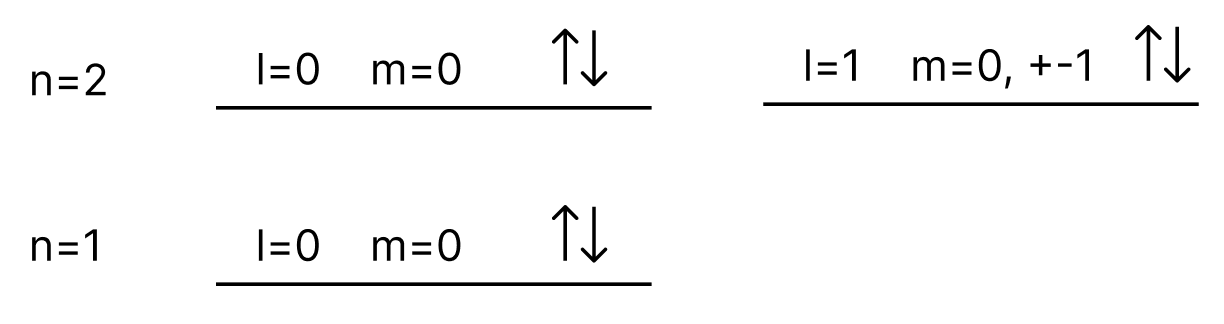
\includegraphics[width=0.5\textwidth]{bozony_fermiony}
    \label{fig:bozony_fermiony}
\end{figure}
\begin{equation*}
    N_e(1s^2, 2s^2, 2p^6)
\end{equation*}
Liczba w wykładniku to liczba elektronów w danym stanie (w danym orbitalu na danym poziomie). Zmienna $n$ numeruje poziomy energetyczne. Na pierwszym
poziomie występuje jeden orbital $1s$, na drugim poziomie występują dwa orbitale $2s$ i $2p$ - mieszczą odpowiednio 2, 2, 6 elektronów. Zmienna $l$ to
orbitalna liczba kwantowa - $0$ odpowiada orbitalowi $s$, $1$ odpowiada orbitalowi $p$, $2$ odpowiada orbitalowi $d$, $3$ odpowiada orbitalowi $f$.
Zmienna $m$ to magnetyczna liczba kwantowa - opisuje orientację orbitalu w przestrzeni. Orbital $s$ ma tylko jedną możliwą orientację,
stąd $m = 0$. Orbital $p$ ma trzy możliwe orientacje, stąd $m = -1, 0, 1$.
\paragraph*{Wniosek}\mbox{}\\
Bez tej zasady świat byłby inny, albo by nie istniał. Bez tej zasady wszystkie elektrony byłyby w tym samym stanie (skondensowałyby się w jednym stanie),
czyli w najniższym stanie energetycznym, co oznaczałoby brak różnorodności pierwiastków chemicznych i stabilnych struktur molekularnych.
%
Zasada Pauliego jest podstawową własnością cząstek.
%
\textbf{Pytanie}: Czym są strzałki góra/dół? Strzałka reprezentuje spin elektronu, który może mieć wartość $m_s = \pm \frac{1}{2}$ (magnetyczna liczba spinowa).


\end{document}
